\documentclass[aspectratio=169]{beamer}
% Shared preamble for ml/ slide decks.
% Each lecture .tex starts with:
%   \documentclass[aspectratio=169]{beamer}
%   % Shared preamble for ml/ slide decks.
% Each lecture .tex starts with:
%   \documentclass[aspectratio=169]{beamer}
%   % Shared preamble for ml/ slide decks.
% Each lecture .tex starts with:
%   \documentclass[aspectratio=169]{beamer}
%   \input{../preamble}
% Compile from inside the chapter folder so \input{../preamble} resolves.

\usetheme{default}
\usecolortheme{dove}

\setbeamertemplate{navigation symbols}{}
\setbeamertemplate{footline}{%
  \hfill{\large\insertframenumber\,/\,\inserttotalframenumber}\hspace{0.8em}\vspace{0.5em}%
}

% Project palette (existing, kept for backwards compatibility with deferred/*)
\definecolor{popblue}{RGB}{52, 101, 164}
\definecolor{sampred}{RGB}{204, 0, 0}
\definecolor{paramgreen}{RGB}{0, 140, 70}
\definecolor{warnred}{RGB}{180, 40, 40}
\definecolor{orange1}{RGB}{220, 120, 0}
\definecolor{violet1}{RGB}{120, 50, 160}
\definecolor{lightbg}{RGB}{245, 245, 250}

% Armenian flag palette (use these for any 3-color highlight; per CLAUDE.md).
% "Nice versions": slightly de-saturated from the official spec for slide use,
% so they don't burn out under projector colors. Originals kept as *_pure.
\definecolor{armred}{RGB}{200, 30, 40}      % nice red (official #D90012 muted)
\definecolor{armblue}{RGB}{30, 70, 160}     % nice blue (official #0033A0 muted)
\definecolor{armorange}{RGB}{230, 160, 30}  % nice orange (official #F2A800 muted)
\definecolor{armred_pure}{HTML}{D90012}     % official Armenian flag red
\definecolor{armblue_pure}{HTML}{0033A0}    % official Armenian flag blue
\definecolor{armorange_pure}{HTML}{F2A800}  % official Armenian flag orange

\setbeamercolor{frametitle}{fg=popblue}
\setbeamercolor{title}{fg=popblue}

\usepackage{pgfplots}
\usepackage{tikz}
\usetikzlibrary{shapes, arrows.meta, positioning, calc, decorations.pathreplacing, patterns, matrix}
\pgfplotsset{compat=1.18}
\usepackage{amsmath, amssymb, amsfonts}
\usepackage{bm}
\usepackage{dsfont}
\usepackage{array}
\usepackage{pifont}
\usepackage{colortbl}
\usepackage{fontenc}

% Callout boxes. Purely additive - existing decks are unaffected.
% Usage: \begin{tcolorbox}[colback=armblue!8, colframe=armblue, boxrule=0.6pt, arc=2pt,
%                          title=\textbf{Key idea}] ... \end{tcolorbox}
% Palette convention (ml/SLIDE_STYLE.md): armblue=key idea, armred=trap/warning,
% paramgreen=takeaway or "Next", armorange=watch-out.
\usepackage[most]{tcolorbox}

% Cleaner table rules (\toprule, \midrule, \bottomrule). Also purely additive.
\usepackage{booktabs}

% \cancel{...} for struck-through terms in derivations (added 2026-08-11 for the
% importance-sampling frame in ch11_rl, where the dynamics cancel). Purely additive.
\usepackage{cancel}

% Minimal ML notation macros (subset of slds-lmu latex-math/basic-ml.tex).
% Kept here so we don't have to inline-expand every \thetav, \xv, etc.
% when porting upstream slides.
\newcommand{\R}{\mathds{R}}
\newcommand{\N}{\mathds{N}}
\newcommand{\E}{\mathds{E}}
\newcommand{\Xspace}{\mathcal{X}}
\newcommand{\Yspace}{\mathcal{Y}}
\newcommand{\Hspace}{\mathcal{H}}
\newcommand{\D}{\mathcal{D}}
\newcommand{\Dtrain}{\mathcal{D}_{\text{train}}}
\newcommand{\Dtest}{\mathcal{D}_{\text{test}}}
\newcommand{\xv}{\mathbf{x}}
\newcommand{\yv}{\mathbf{y}}
\newcommand{\Xmat}{\mathbf{X}}
\newcommand{\id}{\mathbf{I}}
\newcommand{\thetav}{\bm{\theta}}
\newcommand{\thetah}{\hat{\bm{\theta}}}
\newcommand{\lamv}{\bm{\lambda}}
\newcommand{\fx}{f(\xv)}
\newcommand{\fxt}{f(\xv \,|\, \bm{\theta})}
\newcommand{\fxi}{f\!\left(\xv^{(i)}\right)}
\newcommand{\fh}{\hat{f}}
\newcommand{\fxh}{\hat{f}(\xv)}
\newcommand{\yh}{\hat{y}}
\newcommand{\yih}{\hat{y}^{(i)}}
% \xi clashes with the Greek letter \xi; write \xv^{(i)} inline instead.
\newcommand{\yi}[1][i]{y^{(#1)}}
\newcommand{\xyi}[1][i]{\left(\xv^{(#1)},\, y^{(#1)}\right)}
\newcommand{\thx}{\bm{\theta}^\top \xv}
\newcommand{\sumin}{\sum_{i=1}^{n}}
\newcommand{\sumjp}{\sum_{j=1}^{p}}
\newcommand{\Lxy}{L\!\left(y, \fx\right)}
\newcommand{\Lxyi}{L\!\left(\yi, \fxi\right)}
\newcommand{\risk}{\mathcal{R}}
\newcommand{\riske}{\mathcal{R}_{\text{emp}}}
\newcommand{\risket}{\mathcal{R}_{\text{emp}}(\bm{\theta})}
\newcommand{\riskt}{\mathcal{R}(\bm{\theta})}
\newcommand{\riskr}{\mathcal{R}_{\text{reg}}}
\newcommand{\argmin}{\mathop{\mathrm{arg\,min}}}
\newcommand{\argmax}{\mathop{\mathrm{arg\,max}}}
\newcommand{\eps}{\varepsilon}

% Compile from inside the chapter folder so % Shared preamble for ml/ slide decks.
% Each lecture .tex starts with:
%   \documentclass[aspectratio=169]{beamer}
%   \input{../preamble}
% Compile from inside the chapter folder so \input{../preamble} resolves.

\usetheme{default}
\usecolortheme{dove}

\setbeamertemplate{navigation symbols}{}
\setbeamertemplate{footline}{%
  \hfill{\large\insertframenumber\,/\,\inserttotalframenumber}\hspace{0.8em}\vspace{0.5em}%
}

% Project palette (existing, kept for backwards compatibility with deferred/*)
\definecolor{popblue}{RGB}{52, 101, 164}
\definecolor{sampred}{RGB}{204, 0, 0}
\definecolor{paramgreen}{RGB}{0, 140, 70}
\definecolor{warnred}{RGB}{180, 40, 40}
\definecolor{orange1}{RGB}{220, 120, 0}
\definecolor{violet1}{RGB}{120, 50, 160}
\definecolor{lightbg}{RGB}{245, 245, 250}

% Armenian flag palette (use these for any 3-color highlight; per CLAUDE.md).
% "Nice versions": slightly de-saturated from the official spec for slide use,
% so they don't burn out under projector colors. Originals kept as *_pure.
\definecolor{armred}{RGB}{200, 30, 40}      % nice red (official #D90012 muted)
\definecolor{armblue}{RGB}{30, 70, 160}     % nice blue (official #0033A0 muted)
\definecolor{armorange}{RGB}{230, 160, 30}  % nice orange (official #F2A800 muted)
\definecolor{armred_pure}{HTML}{D90012}     % official Armenian flag red
\definecolor{armblue_pure}{HTML}{0033A0}    % official Armenian flag blue
\definecolor{armorange_pure}{HTML}{F2A800}  % official Armenian flag orange

\setbeamercolor{frametitle}{fg=popblue}
\setbeamercolor{title}{fg=popblue}

\usepackage{pgfplots}
\usepackage{tikz}
\usetikzlibrary{shapes, arrows.meta, positioning, calc, decorations.pathreplacing, patterns, matrix}
\pgfplotsset{compat=1.18}
\usepackage{amsmath, amssymb, amsfonts}
\usepackage{bm}
\usepackage{dsfont}
\usepackage{array}
\usepackage{pifont}
\usepackage{colortbl}
\usepackage{fontenc}

% Callout boxes. Purely additive - existing decks are unaffected.
% Usage: \begin{tcolorbox}[colback=armblue!8, colframe=armblue, boxrule=0.6pt, arc=2pt,
%                          title=\textbf{Key idea}] ... \end{tcolorbox}
% Palette convention (ml/SLIDE_STYLE.md): armblue=key idea, armred=trap/warning,
% paramgreen=takeaway or "Next", armorange=watch-out.
\usepackage[most]{tcolorbox}

% Cleaner table rules (\toprule, \midrule, \bottomrule). Also purely additive.
\usepackage{booktabs}

% \cancel{...} for struck-through terms in derivations (added 2026-08-11 for the
% importance-sampling frame in ch11_rl, where the dynamics cancel). Purely additive.
\usepackage{cancel}

% Minimal ML notation macros (subset of slds-lmu latex-math/basic-ml.tex).
% Kept here so we don't have to inline-expand every \thetav, \xv, etc.
% when porting upstream slides.
\newcommand{\R}{\mathds{R}}
\newcommand{\N}{\mathds{N}}
\newcommand{\E}{\mathds{E}}
\newcommand{\Xspace}{\mathcal{X}}
\newcommand{\Yspace}{\mathcal{Y}}
\newcommand{\Hspace}{\mathcal{H}}
\newcommand{\D}{\mathcal{D}}
\newcommand{\Dtrain}{\mathcal{D}_{\text{train}}}
\newcommand{\Dtest}{\mathcal{D}_{\text{test}}}
\newcommand{\xv}{\mathbf{x}}
\newcommand{\yv}{\mathbf{y}}
\newcommand{\Xmat}{\mathbf{X}}
\newcommand{\id}{\mathbf{I}}
\newcommand{\thetav}{\bm{\theta}}
\newcommand{\thetah}{\hat{\bm{\theta}}}
\newcommand{\lamv}{\bm{\lambda}}
\newcommand{\fx}{f(\xv)}
\newcommand{\fxt}{f(\xv \,|\, \bm{\theta})}
\newcommand{\fxi}{f\!\left(\xv^{(i)}\right)}
\newcommand{\fh}{\hat{f}}
\newcommand{\fxh}{\hat{f}(\xv)}
\newcommand{\yh}{\hat{y}}
\newcommand{\yih}{\hat{y}^{(i)}}
% \xi clashes with the Greek letter \xi; write \xv^{(i)} inline instead.
\newcommand{\yi}[1][i]{y^{(#1)}}
\newcommand{\xyi}[1][i]{\left(\xv^{(#1)},\, y^{(#1)}\right)}
\newcommand{\thx}{\bm{\theta}^\top \xv}
\newcommand{\sumin}{\sum_{i=1}^{n}}
\newcommand{\sumjp}{\sum_{j=1}^{p}}
\newcommand{\Lxy}{L\!\left(y, \fx\right)}
\newcommand{\Lxyi}{L\!\left(\yi, \fxi\right)}
\newcommand{\risk}{\mathcal{R}}
\newcommand{\riske}{\mathcal{R}_{\text{emp}}}
\newcommand{\risket}{\mathcal{R}_{\text{emp}}(\bm{\theta})}
\newcommand{\riskt}{\mathcal{R}(\bm{\theta})}
\newcommand{\riskr}{\mathcal{R}_{\text{reg}}}
\newcommand{\argmin}{\mathop{\mathrm{arg\,min}}}
\newcommand{\argmax}{\mathop{\mathrm{arg\,max}}}
\newcommand{\eps}{\varepsilon}
 resolves.

\usetheme{default}
\usecolortheme{dove}

\setbeamertemplate{navigation symbols}{}
\setbeamertemplate{footline}{%
  \hfill{\large\insertframenumber\,/\,\inserttotalframenumber}\hspace{0.8em}\vspace{0.5em}%
}

% Project palette (existing, kept for backwards compatibility with deferred/*)
\definecolor{popblue}{RGB}{52, 101, 164}
\definecolor{sampred}{RGB}{204, 0, 0}
\definecolor{paramgreen}{RGB}{0, 140, 70}
\definecolor{warnred}{RGB}{180, 40, 40}
\definecolor{orange1}{RGB}{220, 120, 0}
\definecolor{violet1}{RGB}{120, 50, 160}
\definecolor{lightbg}{RGB}{245, 245, 250}

% Armenian flag palette (use these for any 3-color highlight; per CLAUDE.md).
% "Nice versions": slightly de-saturated from the official spec for slide use,
% so they don't burn out under projector colors. Originals kept as *_pure.
\definecolor{armred}{RGB}{200, 30, 40}      % nice red (official #D90012 muted)
\definecolor{armblue}{RGB}{30, 70, 160}     % nice blue (official #0033A0 muted)
\definecolor{armorange}{RGB}{230, 160, 30}  % nice orange (official #F2A800 muted)
\definecolor{armred_pure}{HTML}{D90012}     % official Armenian flag red
\definecolor{armblue_pure}{HTML}{0033A0}    % official Armenian flag blue
\definecolor{armorange_pure}{HTML}{F2A800}  % official Armenian flag orange

\setbeamercolor{frametitle}{fg=popblue}
\setbeamercolor{title}{fg=popblue}

\usepackage{pgfplots}
\usepackage{tikz}
\usetikzlibrary{shapes, arrows.meta, positioning, calc, decorations.pathreplacing, patterns, matrix}
\pgfplotsset{compat=1.18}
\usepackage{amsmath, amssymb, amsfonts}
\usepackage{bm}
\usepackage{dsfont}
\usepackage{array}
\usepackage{pifont}
\usepackage{colortbl}
\usepackage{fontenc}

% Callout boxes. Purely additive - existing decks are unaffected.
% Usage: \begin{tcolorbox}[colback=armblue!8, colframe=armblue, boxrule=0.6pt, arc=2pt,
%                          title=\textbf{Key idea}] ... \end{tcolorbox}
% Palette convention (ml/SLIDE_STYLE.md): armblue=key idea, armred=trap/warning,
% paramgreen=takeaway or "Next", armorange=watch-out.
\usepackage[most]{tcolorbox}

% Cleaner table rules (\toprule, \midrule, \bottomrule). Also purely additive.
\usepackage{booktabs}

% \cancel{...} for struck-through terms in derivations (added 2026-08-11 for the
% importance-sampling frame in ch11_rl, where the dynamics cancel). Purely additive.
\usepackage{cancel}

% Minimal ML notation macros (subset of slds-lmu latex-math/basic-ml.tex).
% Kept here so we don't have to inline-expand every \thetav, \xv, etc.
% when porting upstream slides.
\newcommand{\R}{\mathds{R}}
\newcommand{\N}{\mathds{N}}
\newcommand{\E}{\mathds{E}}
\newcommand{\Xspace}{\mathcal{X}}
\newcommand{\Yspace}{\mathcal{Y}}
\newcommand{\Hspace}{\mathcal{H}}
\newcommand{\D}{\mathcal{D}}
\newcommand{\Dtrain}{\mathcal{D}_{\text{train}}}
\newcommand{\Dtest}{\mathcal{D}_{\text{test}}}
\newcommand{\xv}{\mathbf{x}}
\newcommand{\yv}{\mathbf{y}}
\newcommand{\Xmat}{\mathbf{X}}
\newcommand{\id}{\mathbf{I}}
\newcommand{\thetav}{\bm{\theta}}
\newcommand{\thetah}{\hat{\bm{\theta}}}
\newcommand{\lamv}{\bm{\lambda}}
\newcommand{\fx}{f(\xv)}
\newcommand{\fxt}{f(\xv \,|\, \bm{\theta})}
\newcommand{\fxi}{f\!\left(\xv^{(i)}\right)}
\newcommand{\fh}{\hat{f}}
\newcommand{\fxh}{\hat{f}(\xv)}
\newcommand{\yh}{\hat{y}}
\newcommand{\yih}{\hat{y}^{(i)}}
% \xi clashes with the Greek letter \xi; write \xv^{(i)} inline instead.
\newcommand{\yi}[1][i]{y^{(#1)}}
\newcommand{\xyi}[1][i]{\left(\xv^{(#1)},\, y^{(#1)}\right)}
\newcommand{\thx}{\bm{\theta}^\top \xv}
\newcommand{\sumin}{\sum_{i=1}^{n}}
\newcommand{\sumjp}{\sum_{j=1}^{p}}
\newcommand{\Lxy}{L\!\left(y, \fx\right)}
\newcommand{\Lxyi}{L\!\left(\yi, \fxi\right)}
\newcommand{\risk}{\mathcal{R}}
\newcommand{\riske}{\mathcal{R}_{\text{emp}}}
\newcommand{\risket}{\mathcal{R}_{\text{emp}}(\bm{\theta})}
\newcommand{\riskt}{\mathcal{R}(\bm{\theta})}
\newcommand{\riskr}{\mathcal{R}_{\text{reg}}}
\newcommand{\argmin}{\mathop{\mathrm{arg\,min}}}
\newcommand{\argmax}{\mathop{\mathrm{arg\,max}}}
\newcommand{\eps}{\varepsilon}

% Compile from inside the chapter folder so % Shared preamble for ml/ slide decks.
% Each lecture .tex starts with:
%   \documentclass[aspectratio=169]{beamer}
%   % Shared preamble for ml/ slide decks.
% Each lecture .tex starts with:
%   \documentclass[aspectratio=169]{beamer}
%   \input{../preamble}
% Compile from inside the chapter folder so \input{../preamble} resolves.

\usetheme{default}
\usecolortheme{dove}

\setbeamertemplate{navigation symbols}{}
\setbeamertemplate{footline}{%
  \hfill{\large\insertframenumber\,/\,\inserttotalframenumber}\hspace{0.8em}\vspace{0.5em}%
}

% Project palette (existing, kept for backwards compatibility with deferred/*)
\definecolor{popblue}{RGB}{52, 101, 164}
\definecolor{sampred}{RGB}{204, 0, 0}
\definecolor{paramgreen}{RGB}{0, 140, 70}
\definecolor{warnred}{RGB}{180, 40, 40}
\definecolor{orange1}{RGB}{220, 120, 0}
\definecolor{violet1}{RGB}{120, 50, 160}
\definecolor{lightbg}{RGB}{245, 245, 250}

% Armenian flag palette (use these for any 3-color highlight; per CLAUDE.md).
% "Nice versions": slightly de-saturated from the official spec for slide use,
% so they don't burn out under projector colors. Originals kept as *_pure.
\definecolor{armred}{RGB}{200, 30, 40}      % nice red (official #D90012 muted)
\definecolor{armblue}{RGB}{30, 70, 160}     % nice blue (official #0033A0 muted)
\definecolor{armorange}{RGB}{230, 160, 30}  % nice orange (official #F2A800 muted)
\definecolor{armred_pure}{HTML}{D90012}     % official Armenian flag red
\definecolor{armblue_pure}{HTML}{0033A0}    % official Armenian flag blue
\definecolor{armorange_pure}{HTML}{F2A800}  % official Armenian flag orange

\setbeamercolor{frametitle}{fg=popblue}
\setbeamercolor{title}{fg=popblue}

\usepackage{pgfplots}
\usepackage{tikz}
\usetikzlibrary{shapes, arrows.meta, positioning, calc, decorations.pathreplacing, patterns, matrix}
\pgfplotsset{compat=1.18}
\usepackage{amsmath, amssymb, amsfonts}
\usepackage{bm}
\usepackage{dsfont}
\usepackage{array}
\usepackage{pifont}
\usepackage{colortbl}
\usepackage{fontenc}

% Callout boxes. Purely additive - existing decks are unaffected.
% Usage: \begin{tcolorbox}[colback=armblue!8, colframe=armblue, boxrule=0.6pt, arc=2pt,
%                          title=\textbf{Key idea}] ... \end{tcolorbox}
% Palette convention (ml/SLIDE_STYLE.md): armblue=key idea, armred=trap/warning,
% paramgreen=takeaway or "Next", armorange=watch-out.
\usepackage[most]{tcolorbox}

% Cleaner table rules (\toprule, \midrule, \bottomrule). Also purely additive.
\usepackage{booktabs}

% \cancel{...} for struck-through terms in derivations (added 2026-08-11 for the
% importance-sampling frame in ch11_rl, where the dynamics cancel). Purely additive.
\usepackage{cancel}

% Minimal ML notation macros (subset of slds-lmu latex-math/basic-ml.tex).
% Kept here so we don't have to inline-expand every \thetav, \xv, etc.
% when porting upstream slides.
\newcommand{\R}{\mathds{R}}
\newcommand{\N}{\mathds{N}}
\newcommand{\E}{\mathds{E}}
\newcommand{\Xspace}{\mathcal{X}}
\newcommand{\Yspace}{\mathcal{Y}}
\newcommand{\Hspace}{\mathcal{H}}
\newcommand{\D}{\mathcal{D}}
\newcommand{\Dtrain}{\mathcal{D}_{\text{train}}}
\newcommand{\Dtest}{\mathcal{D}_{\text{test}}}
\newcommand{\xv}{\mathbf{x}}
\newcommand{\yv}{\mathbf{y}}
\newcommand{\Xmat}{\mathbf{X}}
\newcommand{\id}{\mathbf{I}}
\newcommand{\thetav}{\bm{\theta}}
\newcommand{\thetah}{\hat{\bm{\theta}}}
\newcommand{\lamv}{\bm{\lambda}}
\newcommand{\fx}{f(\xv)}
\newcommand{\fxt}{f(\xv \,|\, \bm{\theta})}
\newcommand{\fxi}{f\!\left(\xv^{(i)}\right)}
\newcommand{\fh}{\hat{f}}
\newcommand{\fxh}{\hat{f}(\xv)}
\newcommand{\yh}{\hat{y}}
\newcommand{\yih}{\hat{y}^{(i)}}
% \xi clashes with the Greek letter \xi; write \xv^{(i)} inline instead.
\newcommand{\yi}[1][i]{y^{(#1)}}
\newcommand{\xyi}[1][i]{\left(\xv^{(#1)},\, y^{(#1)}\right)}
\newcommand{\thx}{\bm{\theta}^\top \xv}
\newcommand{\sumin}{\sum_{i=1}^{n}}
\newcommand{\sumjp}{\sum_{j=1}^{p}}
\newcommand{\Lxy}{L\!\left(y, \fx\right)}
\newcommand{\Lxyi}{L\!\left(\yi, \fxi\right)}
\newcommand{\risk}{\mathcal{R}}
\newcommand{\riske}{\mathcal{R}_{\text{emp}}}
\newcommand{\risket}{\mathcal{R}_{\text{emp}}(\bm{\theta})}
\newcommand{\riskt}{\mathcal{R}(\bm{\theta})}
\newcommand{\riskr}{\mathcal{R}_{\text{reg}}}
\newcommand{\argmin}{\mathop{\mathrm{arg\,min}}}
\newcommand{\argmax}{\mathop{\mathrm{arg\,max}}}
\newcommand{\eps}{\varepsilon}

% Compile from inside the chapter folder so % Shared preamble for ml/ slide decks.
% Each lecture .tex starts with:
%   \documentclass[aspectratio=169]{beamer}
%   \input{../preamble}
% Compile from inside the chapter folder so \input{../preamble} resolves.

\usetheme{default}
\usecolortheme{dove}

\setbeamertemplate{navigation symbols}{}
\setbeamertemplate{footline}{%
  \hfill{\large\insertframenumber\,/\,\inserttotalframenumber}\hspace{0.8em}\vspace{0.5em}%
}

% Project palette (existing, kept for backwards compatibility with deferred/*)
\definecolor{popblue}{RGB}{52, 101, 164}
\definecolor{sampred}{RGB}{204, 0, 0}
\definecolor{paramgreen}{RGB}{0, 140, 70}
\definecolor{warnred}{RGB}{180, 40, 40}
\definecolor{orange1}{RGB}{220, 120, 0}
\definecolor{violet1}{RGB}{120, 50, 160}
\definecolor{lightbg}{RGB}{245, 245, 250}

% Armenian flag palette (use these for any 3-color highlight; per CLAUDE.md).
% "Nice versions": slightly de-saturated from the official spec for slide use,
% so they don't burn out under projector colors. Originals kept as *_pure.
\definecolor{armred}{RGB}{200, 30, 40}      % nice red (official #D90012 muted)
\definecolor{armblue}{RGB}{30, 70, 160}     % nice blue (official #0033A0 muted)
\definecolor{armorange}{RGB}{230, 160, 30}  % nice orange (official #F2A800 muted)
\definecolor{armred_pure}{HTML}{D90012}     % official Armenian flag red
\definecolor{armblue_pure}{HTML}{0033A0}    % official Armenian flag blue
\definecolor{armorange_pure}{HTML}{F2A800}  % official Armenian flag orange

\setbeamercolor{frametitle}{fg=popblue}
\setbeamercolor{title}{fg=popblue}

\usepackage{pgfplots}
\usepackage{tikz}
\usetikzlibrary{shapes, arrows.meta, positioning, calc, decorations.pathreplacing, patterns, matrix}
\pgfplotsset{compat=1.18}
\usepackage{amsmath, amssymb, amsfonts}
\usepackage{bm}
\usepackage{dsfont}
\usepackage{array}
\usepackage{pifont}
\usepackage{colortbl}
\usepackage{fontenc}

% Callout boxes. Purely additive - existing decks are unaffected.
% Usage: \begin{tcolorbox}[colback=armblue!8, colframe=armblue, boxrule=0.6pt, arc=2pt,
%                          title=\textbf{Key idea}] ... \end{tcolorbox}
% Palette convention (ml/SLIDE_STYLE.md): armblue=key idea, armred=trap/warning,
% paramgreen=takeaway or "Next", armorange=watch-out.
\usepackage[most]{tcolorbox}

% Cleaner table rules (\toprule, \midrule, \bottomrule). Also purely additive.
\usepackage{booktabs}

% \cancel{...} for struck-through terms in derivations (added 2026-08-11 for the
% importance-sampling frame in ch11_rl, where the dynamics cancel). Purely additive.
\usepackage{cancel}

% Minimal ML notation macros (subset of slds-lmu latex-math/basic-ml.tex).
% Kept here so we don't have to inline-expand every \thetav, \xv, etc.
% when porting upstream slides.
\newcommand{\R}{\mathds{R}}
\newcommand{\N}{\mathds{N}}
\newcommand{\E}{\mathds{E}}
\newcommand{\Xspace}{\mathcal{X}}
\newcommand{\Yspace}{\mathcal{Y}}
\newcommand{\Hspace}{\mathcal{H}}
\newcommand{\D}{\mathcal{D}}
\newcommand{\Dtrain}{\mathcal{D}_{\text{train}}}
\newcommand{\Dtest}{\mathcal{D}_{\text{test}}}
\newcommand{\xv}{\mathbf{x}}
\newcommand{\yv}{\mathbf{y}}
\newcommand{\Xmat}{\mathbf{X}}
\newcommand{\id}{\mathbf{I}}
\newcommand{\thetav}{\bm{\theta}}
\newcommand{\thetah}{\hat{\bm{\theta}}}
\newcommand{\lamv}{\bm{\lambda}}
\newcommand{\fx}{f(\xv)}
\newcommand{\fxt}{f(\xv \,|\, \bm{\theta})}
\newcommand{\fxi}{f\!\left(\xv^{(i)}\right)}
\newcommand{\fh}{\hat{f}}
\newcommand{\fxh}{\hat{f}(\xv)}
\newcommand{\yh}{\hat{y}}
\newcommand{\yih}{\hat{y}^{(i)}}
% \xi clashes with the Greek letter \xi; write \xv^{(i)} inline instead.
\newcommand{\yi}[1][i]{y^{(#1)}}
\newcommand{\xyi}[1][i]{\left(\xv^{(#1)},\, y^{(#1)}\right)}
\newcommand{\thx}{\bm{\theta}^\top \xv}
\newcommand{\sumin}{\sum_{i=1}^{n}}
\newcommand{\sumjp}{\sum_{j=1}^{p}}
\newcommand{\Lxy}{L\!\left(y, \fx\right)}
\newcommand{\Lxyi}{L\!\left(\yi, \fxi\right)}
\newcommand{\risk}{\mathcal{R}}
\newcommand{\riske}{\mathcal{R}_{\text{emp}}}
\newcommand{\risket}{\mathcal{R}_{\text{emp}}(\bm{\theta})}
\newcommand{\riskt}{\mathcal{R}(\bm{\theta})}
\newcommand{\riskr}{\mathcal{R}_{\text{reg}}}
\newcommand{\argmin}{\mathop{\mathrm{arg\,min}}}
\newcommand{\argmax}{\mathop{\mathrm{arg\,max}}}
\newcommand{\eps}{\varepsilon}
 resolves.

\usetheme{default}
\usecolortheme{dove}

\setbeamertemplate{navigation symbols}{}
\setbeamertemplate{footline}{%
  \hfill{\large\insertframenumber\,/\,\inserttotalframenumber}\hspace{0.8em}\vspace{0.5em}%
}

% Project palette (existing, kept for backwards compatibility with deferred/*)
\definecolor{popblue}{RGB}{52, 101, 164}
\definecolor{sampred}{RGB}{204, 0, 0}
\definecolor{paramgreen}{RGB}{0, 140, 70}
\definecolor{warnred}{RGB}{180, 40, 40}
\definecolor{orange1}{RGB}{220, 120, 0}
\definecolor{violet1}{RGB}{120, 50, 160}
\definecolor{lightbg}{RGB}{245, 245, 250}

% Armenian flag palette (use these for any 3-color highlight; per CLAUDE.md).
% "Nice versions": slightly de-saturated from the official spec for slide use,
% so they don't burn out under projector colors. Originals kept as *_pure.
\definecolor{armred}{RGB}{200, 30, 40}      % nice red (official #D90012 muted)
\definecolor{armblue}{RGB}{30, 70, 160}     % nice blue (official #0033A0 muted)
\definecolor{armorange}{RGB}{230, 160, 30}  % nice orange (official #F2A800 muted)
\definecolor{armred_pure}{HTML}{D90012}     % official Armenian flag red
\definecolor{armblue_pure}{HTML}{0033A0}    % official Armenian flag blue
\definecolor{armorange_pure}{HTML}{F2A800}  % official Armenian flag orange

\setbeamercolor{frametitle}{fg=popblue}
\setbeamercolor{title}{fg=popblue}

\usepackage{pgfplots}
\usepackage{tikz}
\usetikzlibrary{shapes, arrows.meta, positioning, calc, decorations.pathreplacing, patterns, matrix}
\pgfplotsset{compat=1.18}
\usepackage{amsmath, amssymb, amsfonts}
\usepackage{bm}
\usepackage{dsfont}
\usepackage{array}
\usepackage{pifont}
\usepackage{colortbl}
\usepackage{fontenc}

% Callout boxes. Purely additive - existing decks are unaffected.
% Usage: \begin{tcolorbox}[colback=armblue!8, colframe=armblue, boxrule=0.6pt, arc=2pt,
%                          title=\textbf{Key idea}] ... \end{tcolorbox}
% Palette convention (ml/SLIDE_STYLE.md): armblue=key idea, armred=trap/warning,
% paramgreen=takeaway or "Next", armorange=watch-out.
\usepackage[most]{tcolorbox}

% Cleaner table rules (\toprule, \midrule, \bottomrule). Also purely additive.
\usepackage{booktabs}

% \cancel{...} for struck-through terms in derivations (added 2026-08-11 for the
% importance-sampling frame in ch11_rl, where the dynamics cancel). Purely additive.
\usepackage{cancel}

% Minimal ML notation macros (subset of slds-lmu latex-math/basic-ml.tex).
% Kept here so we don't have to inline-expand every \thetav, \xv, etc.
% when porting upstream slides.
\newcommand{\R}{\mathds{R}}
\newcommand{\N}{\mathds{N}}
\newcommand{\E}{\mathds{E}}
\newcommand{\Xspace}{\mathcal{X}}
\newcommand{\Yspace}{\mathcal{Y}}
\newcommand{\Hspace}{\mathcal{H}}
\newcommand{\D}{\mathcal{D}}
\newcommand{\Dtrain}{\mathcal{D}_{\text{train}}}
\newcommand{\Dtest}{\mathcal{D}_{\text{test}}}
\newcommand{\xv}{\mathbf{x}}
\newcommand{\yv}{\mathbf{y}}
\newcommand{\Xmat}{\mathbf{X}}
\newcommand{\id}{\mathbf{I}}
\newcommand{\thetav}{\bm{\theta}}
\newcommand{\thetah}{\hat{\bm{\theta}}}
\newcommand{\lamv}{\bm{\lambda}}
\newcommand{\fx}{f(\xv)}
\newcommand{\fxt}{f(\xv \,|\, \bm{\theta})}
\newcommand{\fxi}{f\!\left(\xv^{(i)}\right)}
\newcommand{\fh}{\hat{f}}
\newcommand{\fxh}{\hat{f}(\xv)}
\newcommand{\yh}{\hat{y}}
\newcommand{\yih}{\hat{y}^{(i)}}
% \xi clashes with the Greek letter \xi; write \xv^{(i)} inline instead.
\newcommand{\yi}[1][i]{y^{(#1)}}
\newcommand{\xyi}[1][i]{\left(\xv^{(#1)},\, y^{(#1)}\right)}
\newcommand{\thx}{\bm{\theta}^\top \xv}
\newcommand{\sumin}{\sum_{i=1}^{n}}
\newcommand{\sumjp}{\sum_{j=1}^{p}}
\newcommand{\Lxy}{L\!\left(y, \fx\right)}
\newcommand{\Lxyi}{L\!\left(\yi, \fxi\right)}
\newcommand{\risk}{\mathcal{R}}
\newcommand{\riske}{\mathcal{R}_{\text{emp}}}
\newcommand{\risket}{\mathcal{R}_{\text{emp}}(\bm{\theta})}
\newcommand{\riskt}{\mathcal{R}(\bm{\theta})}
\newcommand{\riskr}{\mathcal{R}_{\text{reg}}}
\newcommand{\argmin}{\mathop{\mathrm{arg\,min}}}
\newcommand{\argmax}{\mathop{\mathrm{arg\,max}}}
\newcommand{\eps}{\varepsilon}
 resolves.

\usetheme{default}
\usecolortheme{dove}

\setbeamertemplate{navigation symbols}{}
\setbeamertemplate{footline}{%
  \hfill{\large\insertframenumber\,/\,\inserttotalframenumber}\hspace{0.8em}\vspace{0.5em}%
}

% Project palette (existing, kept for backwards compatibility with deferred/*)
\definecolor{popblue}{RGB}{52, 101, 164}
\definecolor{sampred}{RGB}{204, 0, 0}
\definecolor{paramgreen}{RGB}{0, 140, 70}
\definecolor{warnred}{RGB}{180, 40, 40}
\definecolor{orange1}{RGB}{220, 120, 0}
\definecolor{violet1}{RGB}{120, 50, 160}
\definecolor{lightbg}{RGB}{245, 245, 250}

% Armenian flag palette (use these for any 3-color highlight; per CLAUDE.md).
% "Nice versions": slightly de-saturated from the official spec for slide use,
% so they don't burn out under projector colors. Originals kept as *_pure.
\definecolor{armred}{RGB}{200, 30, 40}      % nice red (official #D90012 muted)
\definecolor{armblue}{RGB}{30, 70, 160}     % nice blue (official #0033A0 muted)
\definecolor{armorange}{RGB}{230, 160, 30}  % nice orange (official #F2A800 muted)
\definecolor{armred_pure}{HTML}{D90012}     % official Armenian flag red
\definecolor{armblue_pure}{HTML}{0033A0}    % official Armenian flag blue
\definecolor{armorange_pure}{HTML}{F2A800}  % official Armenian flag orange

\setbeamercolor{frametitle}{fg=popblue}
\setbeamercolor{title}{fg=popblue}

\usepackage{pgfplots}
\usepackage{tikz}
\usetikzlibrary{shapes, arrows.meta, positioning, calc, decorations.pathreplacing, patterns, matrix}
\pgfplotsset{compat=1.18}
\usepackage{amsmath, amssymb, amsfonts}
\usepackage{bm}
\usepackage{dsfont}
\usepackage{array}
\usepackage{pifont}
\usepackage{colortbl}
\usepackage{fontenc}

% Callout boxes. Purely additive - existing decks are unaffected.
% Usage: \begin{tcolorbox}[colback=armblue!8, colframe=armblue, boxrule=0.6pt, arc=2pt,
%                          title=\textbf{Key idea}] ... \end{tcolorbox}
% Palette convention (ml/SLIDE_STYLE.md): armblue=key idea, armred=trap/warning,
% paramgreen=takeaway or "Next", armorange=watch-out.
\usepackage[most]{tcolorbox}

% Cleaner table rules (\toprule, \midrule, \bottomrule). Also purely additive.
\usepackage{booktabs}

% \cancel{...} for struck-through terms in derivations (added 2026-08-11 for the
% importance-sampling frame in ch11_rl, where the dynamics cancel). Purely additive.
\usepackage{cancel}

% Minimal ML notation macros (subset of slds-lmu latex-math/basic-ml.tex).
% Kept here so we don't have to inline-expand every \thetav, \xv, etc.
% when porting upstream slides.
\newcommand{\R}{\mathds{R}}
\newcommand{\N}{\mathds{N}}
\newcommand{\E}{\mathds{E}}
\newcommand{\Xspace}{\mathcal{X}}
\newcommand{\Yspace}{\mathcal{Y}}
\newcommand{\Hspace}{\mathcal{H}}
\newcommand{\D}{\mathcal{D}}
\newcommand{\Dtrain}{\mathcal{D}_{\text{train}}}
\newcommand{\Dtest}{\mathcal{D}_{\text{test}}}
\newcommand{\xv}{\mathbf{x}}
\newcommand{\yv}{\mathbf{y}}
\newcommand{\Xmat}{\mathbf{X}}
\newcommand{\id}{\mathbf{I}}
\newcommand{\thetav}{\bm{\theta}}
\newcommand{\thetah}{\hat{\bm{\theta}}}
\newcommand{\lamv}{\bm{\lambda}}
\newcommand{\fx}{f(\xv)}
\newcommand{\fxt}{f(\xv \,|\, \bm{\theta})}
\newcommand{\fxi}{f\!\left(\xv^{(i)}\right)}
\newcommand{\fh}{\hat{f}}
\newcommand{\fxh}{\hat{f}(\xv)}
\newcommand{\yh}{\hat{y}}
\newcommand{\yih}{\hat{y}^{(i)}}
% \xi clashes with the Greek letter \xi; write \xv^{(i)} inline instead.
\newcommand{\yi}[1][i]{y^{(#1)}}
\newcommand{\xyi}[1][i]{\left(\xv^{(#1)},\, y^{(#1)}\right)}
\newcommand{\thx}{\bm{\theta}^\top \xv}
\newcommand{\sumin}{\sum_{i=1}^{n}}
\newcommand{\sumjp}{\sum_{j=1}^{p}}
\newcommand{\Lxy}{L\!\left(y, \fx\right)}
\newcommand{\Lxyi}{L\!\left(\yi, \fxi\right)}
\newcommand{\risk}{\mathcal{R}}
\newcommand{\riske}{\mathcal{R}_{\text{emp}}}
\newcommand{\risket}{\mathcal{R}_{\text{emp}}(\bm{\theta})}
\newcommand{\riskt}{\mathcal{R}(\bm{\theta})}
\newcommand{\riskr}{\mathcal{R}_{\text{reg}}}
\newcommand{\argmin}{\mathop{\mathrm{arg\,min}}}
\newcommand{\argmax}{\mathop{\mathrm{arg\,max}}}
\newcommand{\eps}{\varepsilon}


\graphicspath{{fig/}{fig/borrowed/}{fig/borrowed/3b1b/}{fig/borrowed/paper/}}

% credit / citation lines (as in LLM-3)
\newcommand{\bbb}{{\scriptsize\color{gray} 3Blue1Brown}}
\newcommand{\paper}[1]{{\scriptsize\color{gray} #1}}

% full-bleed 3Blue1Brown still with a one-line caption pinned near the bottom. Wrapped in a group
% so the background template reverts after this one [plain] frame. Needs 2 pdflatex passes.
\newcommand{\bbbcap}[2]{%
  {\usebackgroundtemplate{\includegraphics[width=\paperwidth,height=\paperheight]{#1}}%
  \begin{frame}[plain]
    \begin{tikzpicture}[remember picture, overlay]
      \node[anchor=south west, font=\tiny, text=white!60]
        at ([shift={(0.26cm,0.16cm)}]current page.south west) {3Blue1Brown};
      \node[anchor=south, font=\small\itshape, text=white, fill=black!60,
            inner sep=5pt, rounded corners, text width=0.86\paperwidth, align=center]
        at ([shift={(0,0.85cm)}]current page.south) {#2};
    \end{tikzpicture}
  \end{frame}}%
}

% callout boxes, matching LLM-1, LLM-2, LLM-3 and LLM-6
\newcommand{\keybox}[1]{\fcolorbox{armblue}{armblue!8}{\parbox{0.97\linewidth}{\small #1}}}
\newcommand{\trapbox}[1]{\fcolorbox{armred}{armred!8}{\parbox{0.97\linewidth}{\small #1}}}
\newcommand{\takebox}[1]{\fcolorbox{paramgreen}{paramgreen!8}{\parbox{0.97\linewidth}{\small #1}}}
\newcommand{\watchbox}[1]{\fcolorbox{armorange}{armorange!12}{\parbox{0.97\linewidth}{\small #1}}}

\newcommand{\sectiontransition}[2]{%
  \begin{frame}[plain]
    \vfill
    \begin{center}
      {\Huge\bfseries\color{popblue} #1}\\[1.1em]
      {\large #2}
    \end{center}
    \vfill
  \end{frame}}

\title{The Transformer block}
\subtitle{Many heads, the MLP, and the residual stream}
\author{}
\date{}

\begin{document}

\begin{frame}[plain]
  \titlepage
  \begin{center}\scriptsize\color{gray}
    LLM chapter, session 4. Parts adapt 3Blue1Brown, ``Deep Learning'' chapters 6 and 7.
  \end{center}
\end{frame}

% ============================================================ WHERE WE ARE (py_src/llm_roadmap.py)
\begin{frame}{Where we are: one forward pass}
  \begin{center}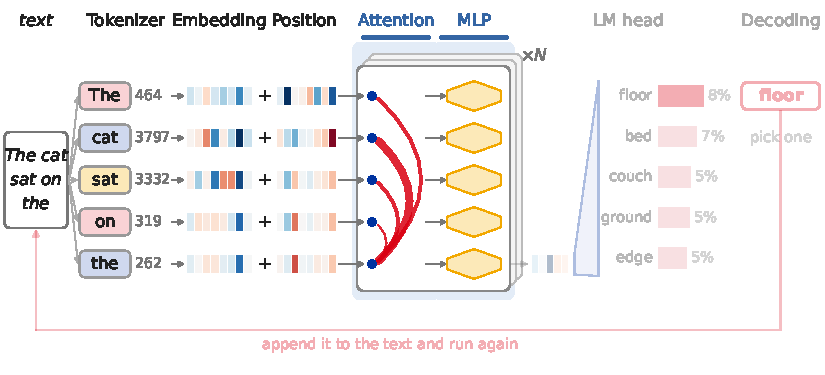
\includegraphics[width=\linewidth]{roadmap_block_pass.pdf}\end{center}
  \vskip -2pt
  {\small Today: the rest of one layer - many heads and the MLP - and why it stacks 12 times.}
\end{frame}

\begin{frame}{Where we are: the life of a model}
  \begin{center}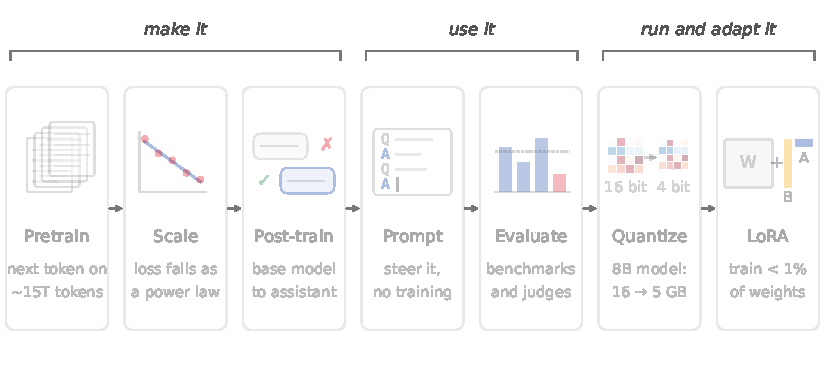
\includegraphics[width=\linewidth]{roadmap_block_life.pdf}\end{center}
  \vskip -2pt
  {\small Later: where these weights come from, and what you do with them once you have them.}
\end{frame}

% ============================================================ COLD OPEN
\begin{frame}{What does GPT-2 write next?}
  \vskip 6pt
  Four prompts for GPT-2 small, the model on our map. Predict its next word:
  \vskip 10pt
  \begin{center}
  \begin{tabular}{l}
    ``Lionel Messi plays the sport of \ldots'' \\[4pt]
    ``Henrikh Mkhitaryan plays the sport of \ldots'' \\[4pt]
    ``Ella Fitzgerald was a famous American \ldots'' \\[4pt]
    ``Elliott Smith was a famous American \ldots'' \\
  \end{tabular}
  \end{center}
  \vskip 12pt
  \keybox{\textbf{Predict:} which of the four does it get right? And for the ones it gets wrong,
  what does it say instead?}
\end{frame}

\begin{frame}{Stored, half-stored, missing}
  \begin{center}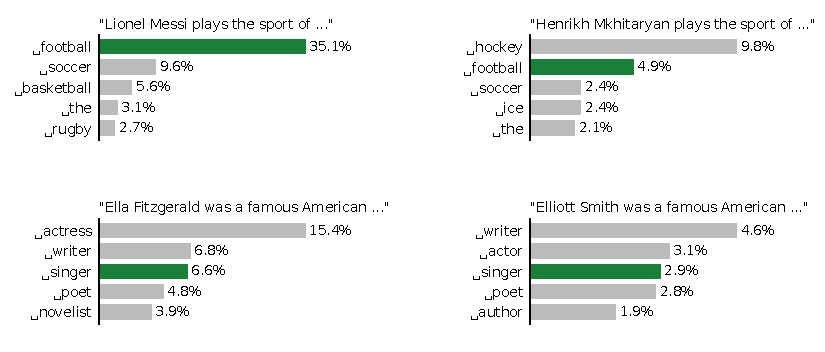
\includegraphics[width=0.94\linewidth]{blk_fact_probes.pdf}\end{center}
  \vskip -4pt
  {\small Messi is stored: football, 35\%. Mkhitaryan is missing: hockey first, football 5\%.
  ``Singer'' is third for both musicians, but 6.6\% against 2.9\%. One run of the real GPT-2.}
\end{frame}

\begin{frame}{So where does a fact live?}
  \vskip 10pt
  No word in these sentences says ``football'' or ``singer''.
  \vskip 8pt
  Attention (LLM-3) only blends what the token vectors already hold. So the fact is either in a
  token's own vector from the start (LLM-2's table), or something adds it on the way through the
  layers.
  \vskip 8pt
  And LLM-1 shows up again: ``Lionel Messi'' is 2 tokens, ``Henrikh Mkhitaryan'' is 7 pieces.
  The model has to put the name together before it can look anything up.
  \vskip 12pt
  \keybox{Today's answer, as far as the evidence goes: mostly in the \textbf{MLP}, the half of
  each layer that LLM-3 never touched - and the bigger half.}
\end{frame}

\begin{frame}{Three things stand between one head and GPT-2}
  \vskip 6pt
  LLM-3 built \textbf{one head}: queries, keys, values, $\mathrm{softmax}(QK^\top/\sqrt{d_k})V$.
  To get from there to one layer of GPT-2:
  \vskip 8pt
  \begin{enumerate}
    \item[\textbf{1.}] \textbf{One head asks one question.} $\to$ many heads.
    \item[\textbf{2.}] \textbf{Tokens talk, but never think alone.} $\to$ the MLP, where facts like
      Messi's sport seem to live.
    \item[\textbf{3.}] \textbf{One layer is not a network.} $\to$ the residual stream and its
      norms; and a model that writes left to right must not read the future $\to$ the mask.
  \end{enumerate}
  \vskip 10pt
  \keybox{The three fixes bolted onto one head of attention \emph{are} the Transformer block.}
\end{frame}

\begin{frame}{Outline}
  \tableofcontents
\end{frame}

% ============================================================ SECTION 1
\section{Many heads}
\sectiontransition{Many heads}{One head asks one question.}

\begin{frame}{By hand: two heads, two questions}
  \begin{columns}[T]
    \column{0.42\textwidth}
    \small
    LLM-3's toy, slots [adjective, fluffy, blue, noun].
    \vskip 4pt
    \textbf{Head 1} asks ``any adjectives?'' (LLM-3's head): weights $0.47, 0.47, 0.06$; it
    hands over fluffiness, $0.47$.
    \vskip 4pt
    \textbf{Head 2} asks ``what colour?'' (its key reads the blue slot): weights
    $0.11, 0.79, 0.11$; it hands over blueness, $0.79$.
    \vskip 4pt
    $W_O$ puts both into the stream: creature gets $(0,\ 0.47,\ 0.79,\ 0)$.
    \column{0.56\textwidth}
    \vskip 6pt
    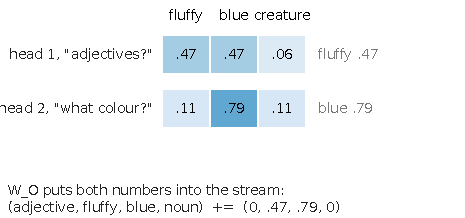
\includegraphics[width=\linewidth]{blk_two_heads.pdf}
  \end{columns}
  \vskip 4pt
  \takebox{Two questions at once; $W_O$ decides where each answer lands. Real heads hand over 64
  numbers each, not one.}
\end{frame}

\begin{frame}{Run it $h$ times, in parallel}
  \vskip 4pt
  Nothing about one head changes. Learn $h$ independent sets of $W_Q, W_K, W_V$, run them at the
  same time, put the outputs side by side, and mix them with one more matrix $W_O$:
  \vskip 6pt
  \begin{center}
  $\text{MultiHead}(X) = \text{Concat}(\text{head}_1, \ldots, \text{head}_h)\, W_O$,
  \qquad $\text{head}_i = \text{Attention}(XW_Q^{(i)}, XW_K^{(i)}, XW_V^{(i)})$
  \end{center}
  \vskip 8pt
  \keybox{\textbf{GPT-2: 12 heads $\times$ 64 numbers $=$ 768}, the size of a token's vector
  (LLM-3's ``why 64''). All twelve heads' $W_Q, W_K, W_V$ sit in one $768 \times 2{,}304$ matrix;
  $W_O$ is $768 \times 768$, so every output number can draw on every head. The same budget as
  one 768-wide head: you \textbf{split} it into 12 views, you do not add any.}
  \vskip 6pt
  {\small The heads do not talk to each other until the concatenation, so all twelve are one big
  batched matrix product.}
\end{frame}

\bbbcap{multihead.png}{Multi-head attention: the same mechanism, many times over, each head free
to learn a different pattern.}

\begin{frame}{Do heads actually specialise, or is that a story?}
  \begin{columns}[T]
    \column{0.52\textwidth}
    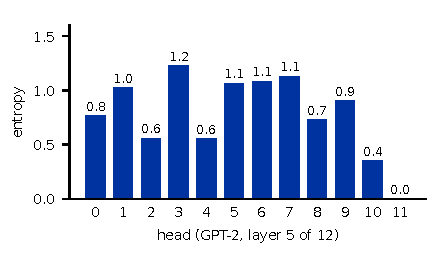
\includegraphics[width=\linewidth]{blk_gpt2_entropy.pdf}
    \column{0.46\textwidth}
    \vskip 6pt
    \small
    Measured: the real GPT-2, the creature sentence, the 12 heads of layer 5.
    \vskip 4pt
    \textbf{Attention entropy} $= -\sum_j a_{ij}\log a_{ij}$, averaged over rows: low means a head
    looks at few tokens, high means it spreads out.
    \vskip 4pt
    Head 11 scores \textbf{0.0}: every token puts all of its weight on a single token. Which one?
    Next slide.
  \end{columns}
\end{frame}

\begin{frame}{Three real heads, one sentence}
  \begin{center}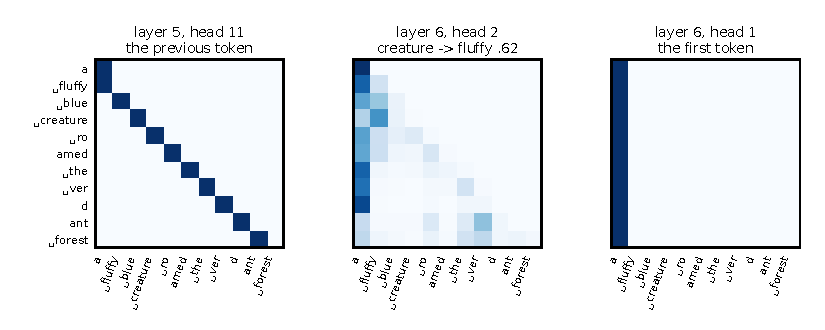
\includegraphics[width=\linewidth]{blk_gpt2_heads.pdf}\end{center}
  \vskip -6pt
  {\small Left: every token looks exactly one token back (weight 1.00) - the head with entropy 0.
  Middle: on this sentence, creature sends 62\% of its attention to fluffy - LLM-3's toy, for
  real. Right: everything goes to the first token, ``a''.}
\end{frame}

\begin{frame}{Attention sinks}
  \begin{columns}[T]
    \column{0.5\textwidth}
    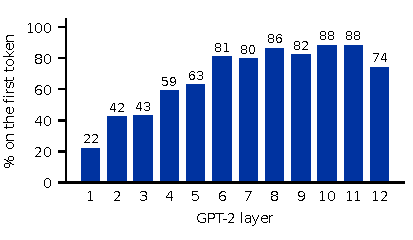
\includegraphics[width=\linewidth]{blk_gpt2_sink.pdf}
    \column{0.48\textwidth}
    \vskip 6pt
    \small
    The right-hand pattern is not rare: \textbf{39 of GPT-2's 144 heads} put over 90\% of their
    attention on the first token of this sentence. The share grows with depth: 22\% in layer 1,
    88\% in layer 10.
    \vskip 6pt
    The usual explanation: softmax must hand out a total of 1, so a head with nothing useful to
    look at parks its weight on one token whose value changes little - the first.
  \end{columns}
  \vskip 6pt
  \watchbox{This is called an \textbf{attention sink} \paper{(Xiao et al., ICLR 2024)}. Real
  heads are messier than the toy, exactly as LLM-3 warned.}
\end{frame}

\begin{frame}{What the specialisations look like}
  \vskip 8pt
  Across models and layers, heads fall into recognisable jobs:
  \vskip 8pt
  \begin{center}
  \small
  \begin{tabular}{ll}
    \toprule
    \textbf{Kind of head} & \textbf{What it attends to} \\
    \midrule
    positional & the previous token, or the first one (both above) \\
    syntactic  & the verb belonging to this subject; the noun this adjective modifies \\
    coreference & the name a pronoun refers to \\
    lexical    & the other half of a multi-token name (\emph{Lionel} $\leftrightarrow$ \emph{Messi}) \\
    \bottomrule
  \end{tabular}
  \end{center}
  \vskip 10pt
  \watchbox{Read these labels with some suspicion. Nobody assigned these jobs; they are patterns
  \emph{we} recognise afterwards, on the sentences we looked at, and plenty of heads do nothing
  so tidy. The measured claim is that the heads differ.}
\end{frame}

\begin{frame}{One head or twelve: still blind to order}
  \begin{center}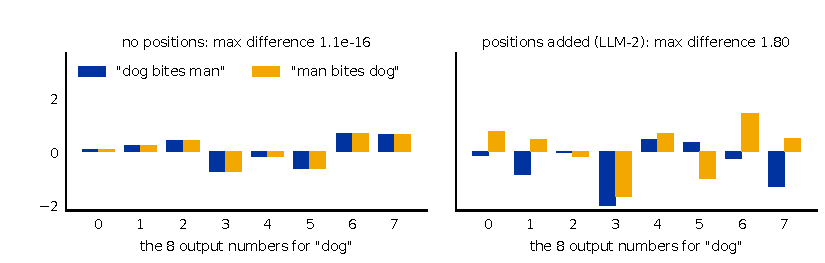
\includegraphics[width=0.92\linewidth]{blk_permutation.pdf}\end{center}
  \vskip -4pt
  {\small The proof LLM-2 promised. Same three word vectors, ``dog bites man'' vs ``man bites
  dog'', one head: ``dog'' gets the same output in both, up to $1.1 \times 10^{-16}$ -
  floating-point zero. Add positions (right) and the two differ.}
  \vskip 4pt
  \keybox{Nowhere for order to enter: $\mathbf{q}_i \cdot \mathbf{k}_j$ uses only the two
  vectors, softmax works on a set, and the output is a sum. Permute the inputs and the outputs
  come back permuted, unchanged. That is why LLM-2 adds positions before the first layer.}
\end{frame}

% ============================================================ SECTION 2
\section{The MLP: where facts live}
\sectiontransition{The MLP: where facts live}{Attention moves information around. Something has to
store it.}

\bbbcap{ch7_mj_hook.jpg}{3Blue1Brown's version of our question: ``Michael Jordan plays the sport
of \_\_\_''. Ours was Messi.}

\begin{frame}{Where the MLP sits}
  \begin{columns}[T]
    \column{0.56\textwidth}
    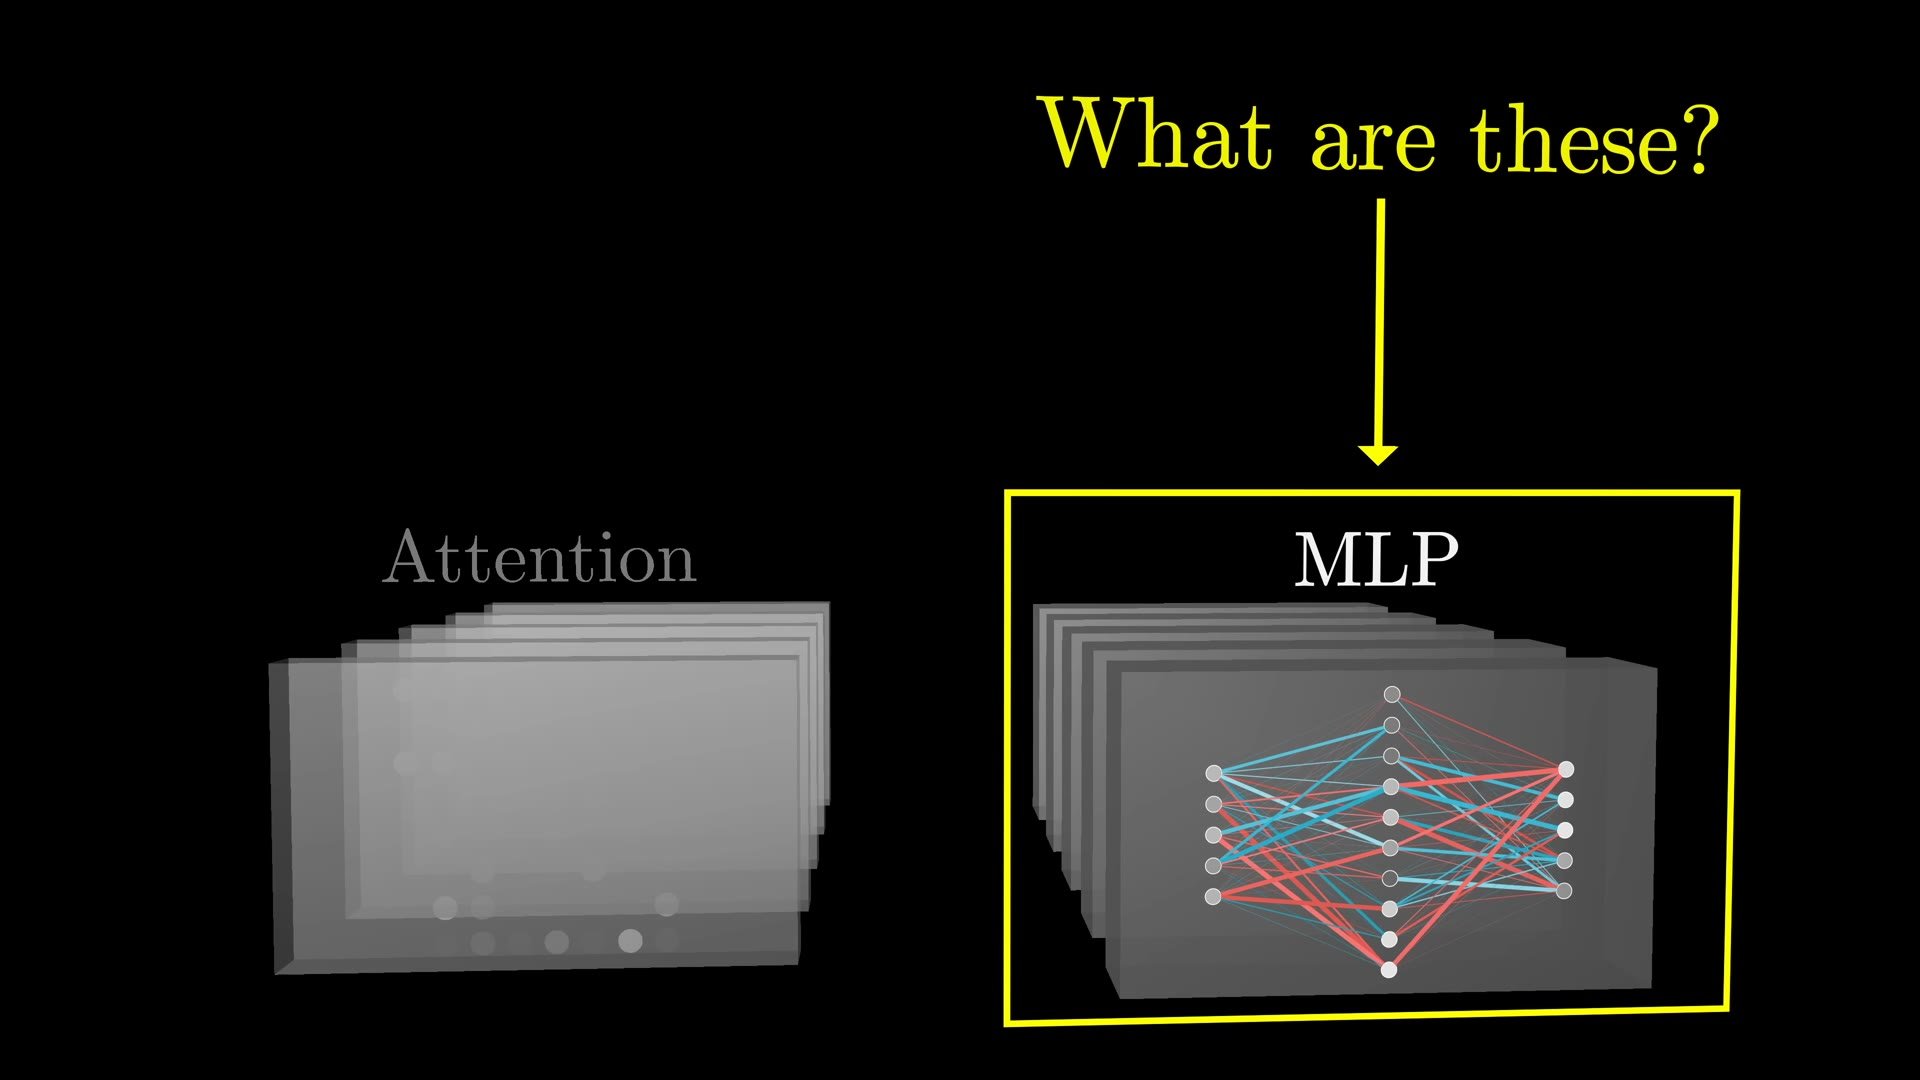
\includegraphics[width=\linewidth]{ch7_flow_mlp.jpg}\\ \bbb
    \column{0.42\textwidth}
    \vskip 6pt
    After attention, every token goes through the \textbf{same} small network, \textbf{alone}:
    no token sees another inside the MLP.
    \vskip 6pt
    It is the network from [41]: a linear layer, a nonlinearity, a linear layer.
    \vskip 6pt
    \keybox{Attention: tokens talk. MLP: each token thinks on its own.}
  \end{columns}
\end{frame}

\begin{frame}{A direction is a question}
  \begin{columns}[T]
    \column{0.56\textwidth}
    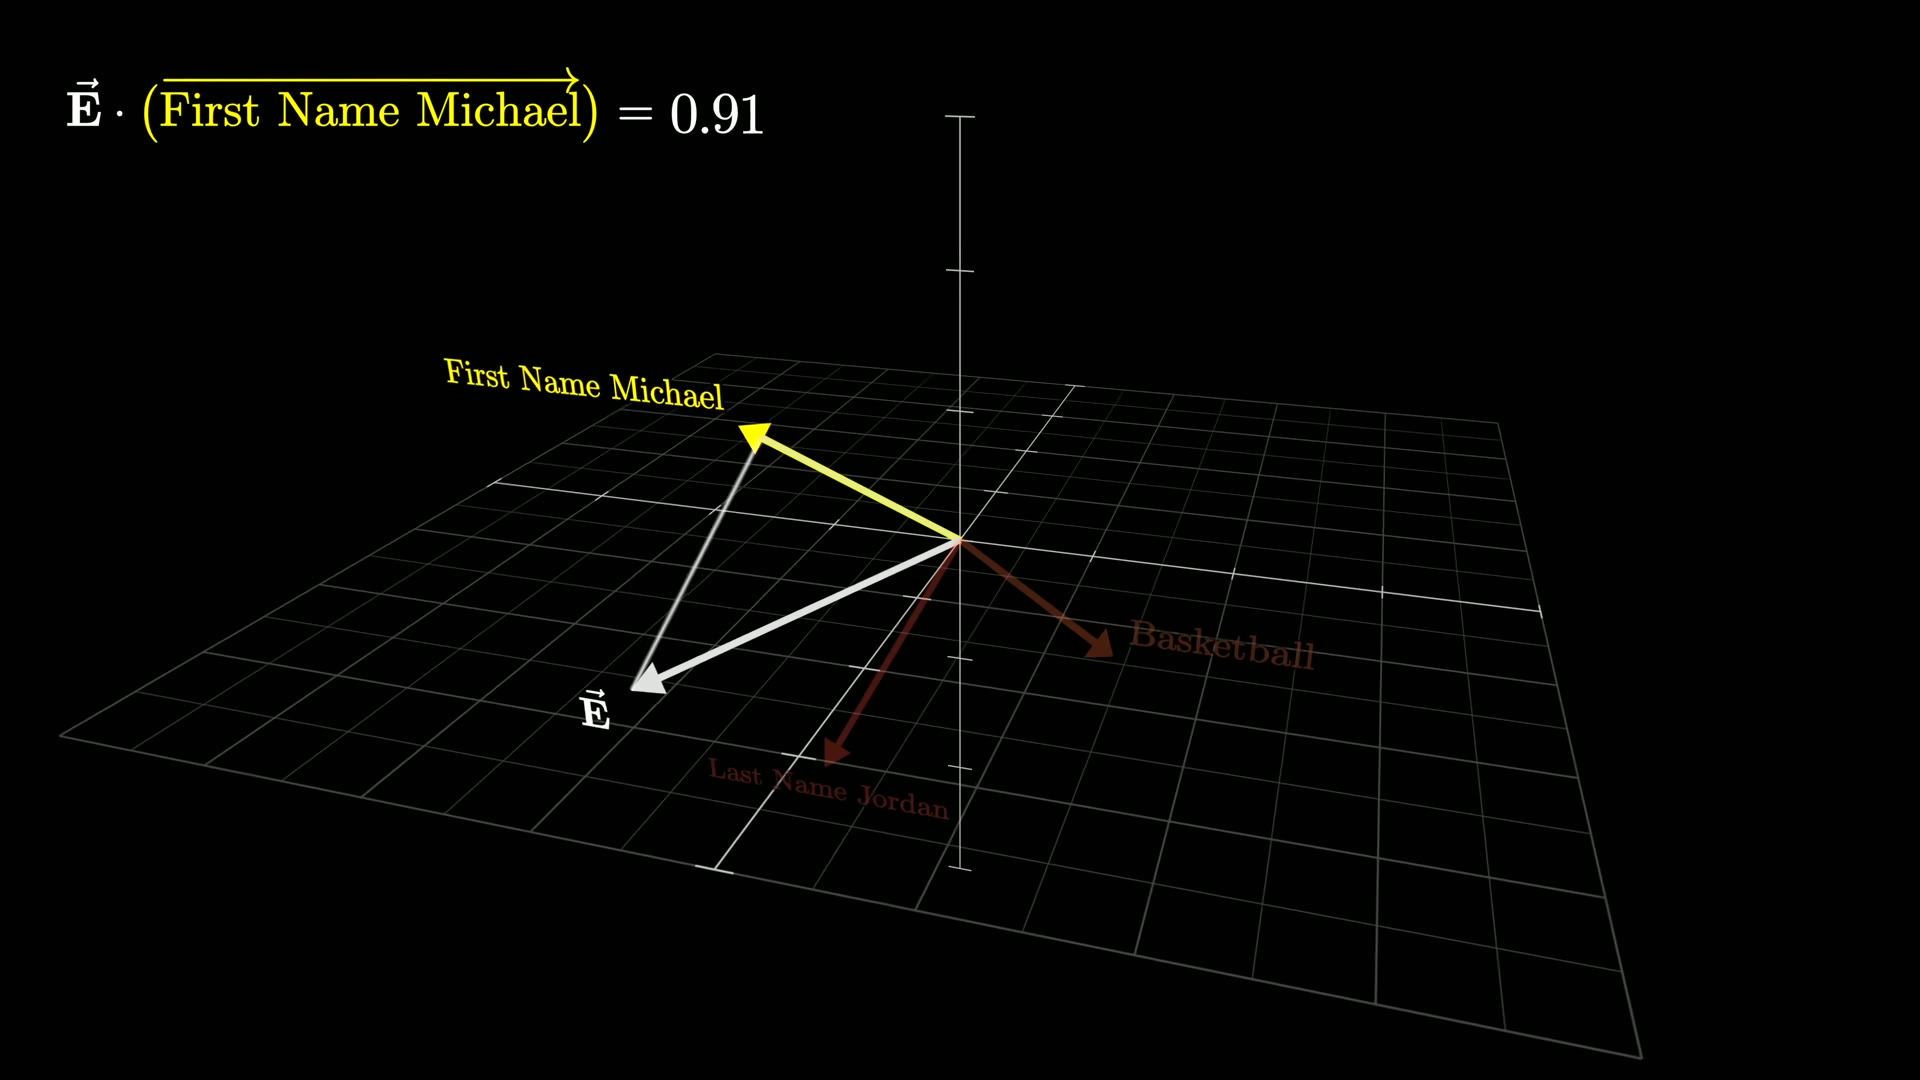
\includegraphics[width=\linewidth]{ch7_direction_dotprod.jpg}\\ \bbb
    \column{0.42\textwidth}
    \vskip 6pt
    LLM-2: directions in the vector space carry meaning. The dot product with a direction
    measures \emph{how much} of that idea a vector holds.
    \vskip 6pt
    Here: how much ``first name Michael'' is in this token's vector? $0.91$: a lot.
  \end{columns}
\end{frame}

\begin{frame}{Up-projection: each row asks a question}
  \begin{columns}[T]
    \column{0.56\textwidth}
    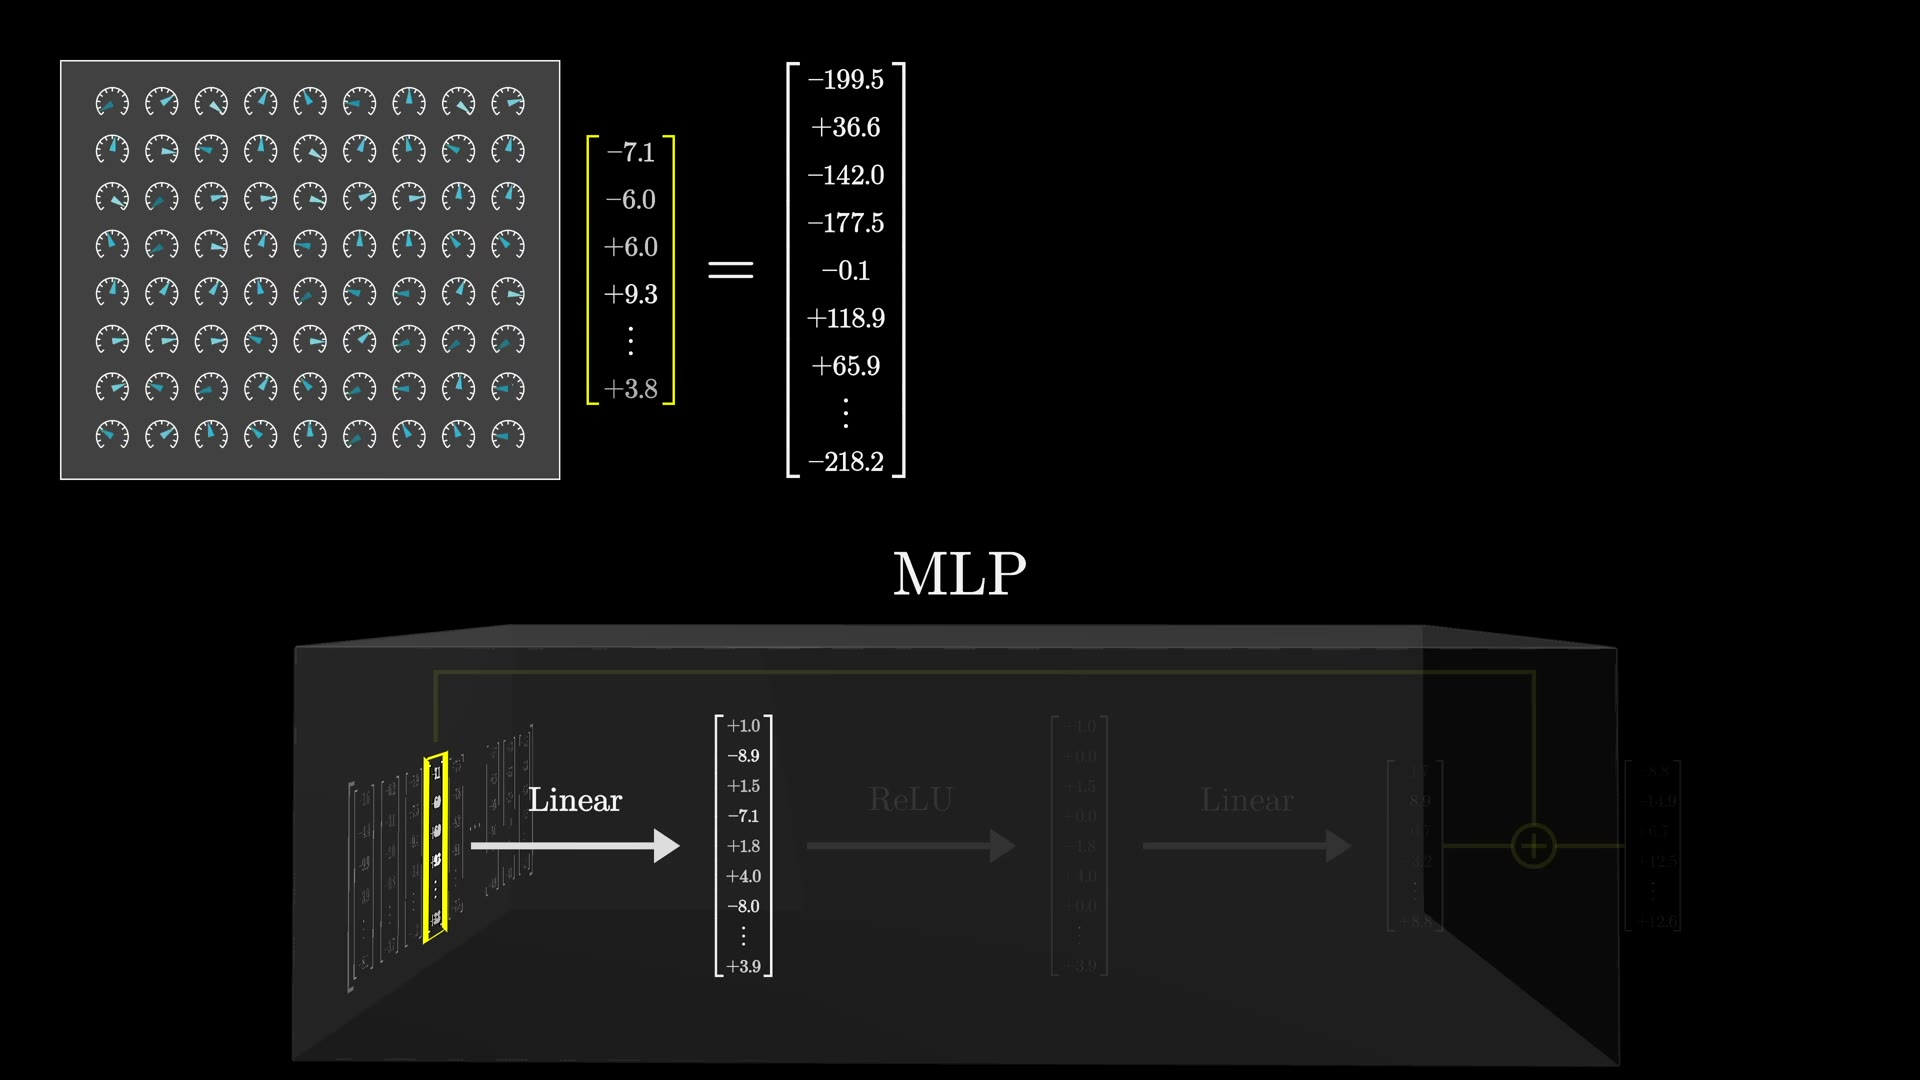
\includegraphics[width=\linewidth]{ch7_upproj_rows.jpg}\\ \bbb
    \column{0.42\textwidth}
    \vskip 6pt
    The first layer computes $W_{\text{up}}\,\mathbf{x} + \mathbf{b}$. Each \textbf{row} of
    $W_{\text{up}}$ is one such question, a dot product with one direction; the bias is a
    threshold.
    \vskip 6pt
    GPT-2 asks \textbf{3{,}072} questions per token: four times its 768 numbers.
  \end{columns}
\end{frame}

\begin{frame}{ReLU makes an AND gate}
  \begin{columns}[T]
    \column{0.56\textwidth}
    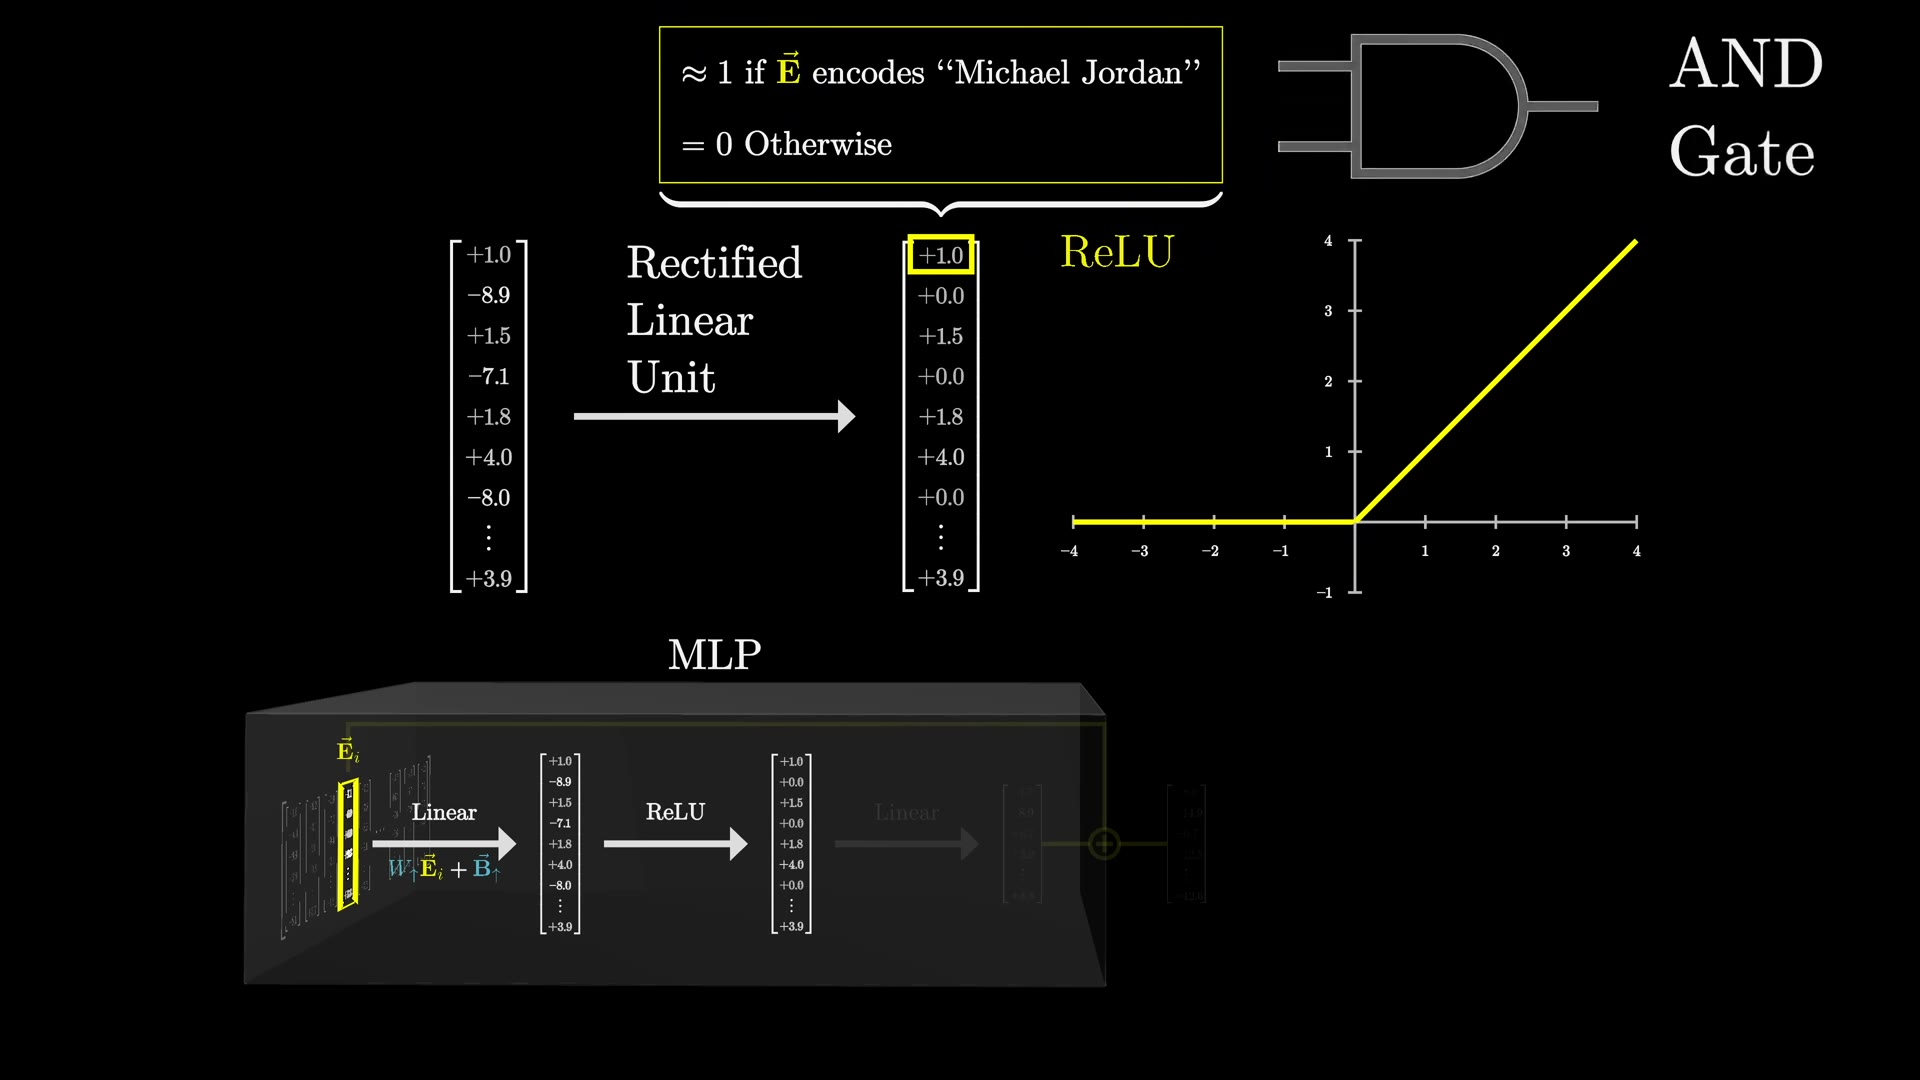
\includegraphics[width=\linewidth]{ch7_relu_andgate.jpg}\\ \bbb
    \column{0.42\textwidth}
    \vskip 6pt
    Ask ``first name Michael'' $+$ ``last name Jordan'', with bias $-1$: the sum is positive only
    if \textbf{both} are there.
    \vskip 6pt
    ReLU sets everything negative to 0. What is left is a neuron that fires on ``Michael AND
    Jordan'' and stays silent otherwise.
    \vskip 6pt
    {\footnotesize GPT-2 actually uses GELU, a smoothed ReLU (slightly negative instead of exactly
    0 below zero); the gate works the same way.}
  \end{columns}
\end{frame}

\begin{frame}{Down-projection: each column adds something}
  \begin{columns}[T]
    \column{0.56\textwidth}
    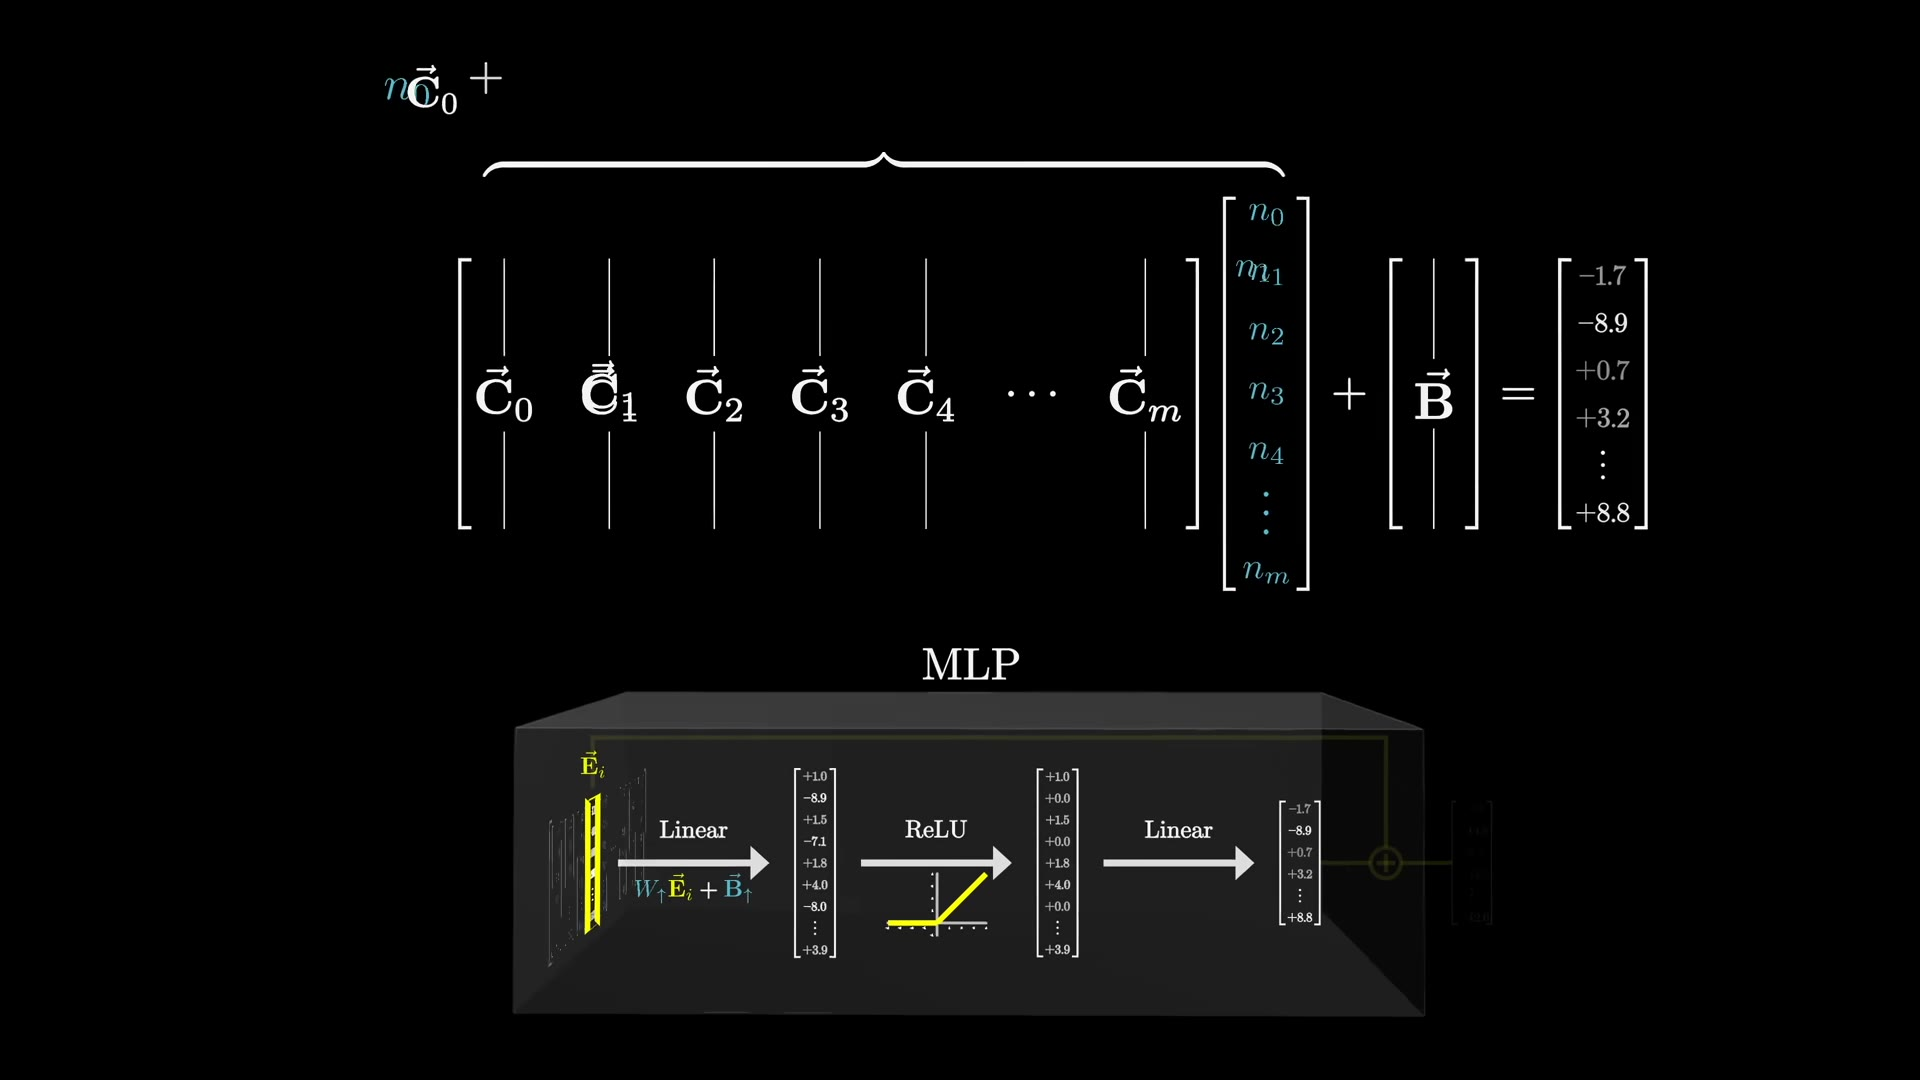
\includegraphics[width=\linewidth]{ch7_downproj_columns.jpg}\\ \bbb
    \column{0.42\textwidth}
    \vskip 6pt
    The second layer maps the 3{,}072 neuron values back to 768 numbers. Each \textbf{column} of
    $W_{\text{down}}$ is a direction; a neuron that fires adds its column into the stream.
    \vskip 6pt
    The ``Michael Jordan'' neuron's column can point toward ``basketball''. The fact is in the
    weights.
  \end{columns}
\end{frame}

\begin{frame}{By hand: a neuron on creature}
  \begin{columns}[T]
    \column{0.5\textwidth}
    \small
    After LLM-3, creature is $(0,\ 0.47,\ 0.47,\ 2.13)$. Give the toy one more slot,
    \textbf{cute}, that every word left at 0 - real vectors have 768 slots, most unnamed.
    \vskip 4pt
    One neuron: $\mathrm{ReLU}(\text{fluffy} + 0.5\,\text{noun} - 1.2)$.
    \begin{itemize}
      \item this creature: $0.47 + 1.065 - 1.2 = \mathbf{0.335}$
      \item a plain creature $(0,0,0,2)$: $-0.2 \to 0$
      \item fluffy alone: $-0.2 \to 0$; blue alone: $-1.2 \to 0$
    \end{itemize}
    Its column writes $3 \times 0.335 = 1.0$ into cute.
    \column{0.48\textwidth}
    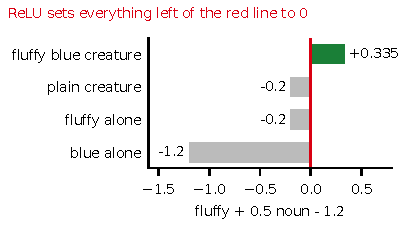
\includegraphics[width=\linewidth]{blk_neuron.pdf}
  \end{columns}
  \vskip 4pt
  \takebox{The neuron fires on ``fluffy AND creature''. That only works because attention first
  brought fluffy into creature's vector (LLM-3) - Michael and Jordan, the same way. Now creature
  carries a feature no word in the sentence had.}
\end{frame}

\bbbcap{ch7_mlp_full.jpg}{The whole MLP: linear, ReLU, linear, then add the result back into the
stream. The same weights for every token.}

\begin{frame}{Two thirds of the weights}
  \begin{center}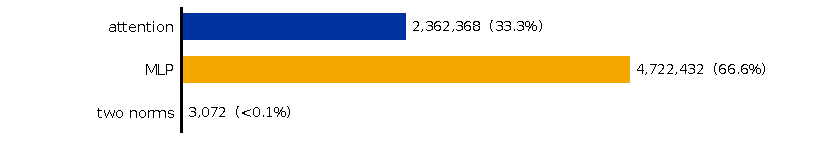
\includegraphics[width=0.9\linewidth]{blk_params_block.pdf}\end{center}
  \vskip -2pt
  {\small One GPT-2 block, counted from its weight file: the MLP holds \textbf{66.6\%}. 3Blue1Brown
  counts the same share for GPT-3. Last lecture was about the smaller half.}
  \vskip 6pt
  \keybox{Evidence that facts sit in these layers: the MLPs behave like key-value memories
  \paper{(Geva et al., EMNLP 2021)}, and editing one mid-layer MLP can change what GPT-2 XL says
  about a fact \paper{(Meng et al., NeurIPS 2022)}. And the cold open: models answer worse about
  people and things that are rare in their training text \paper{(Kandpal et al., ICML 2023)}.}
\end{frame}

\begin{frame}{More facts than dimensions?}
  \begin{columns}[T]
    \column{0.52\textwidth}
    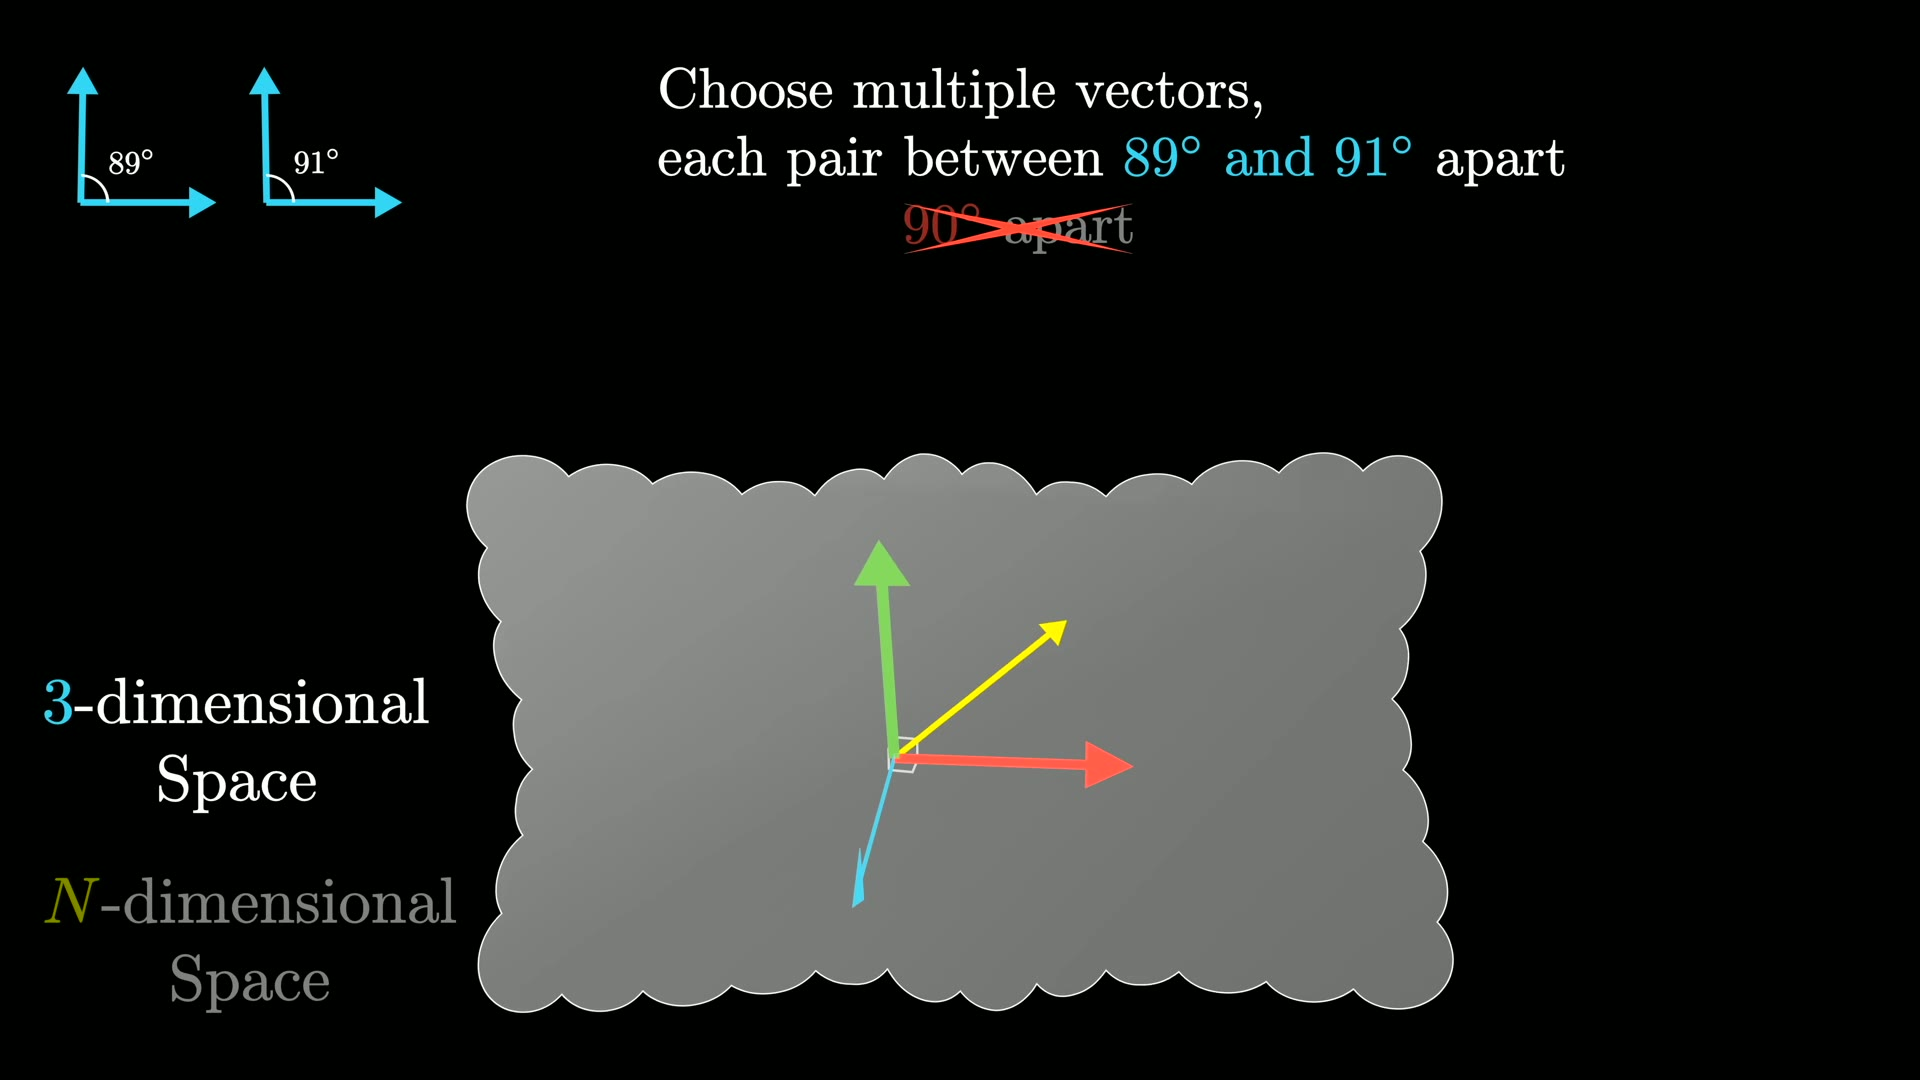
\includegraphics[width=\linewidth]{ch7_nearly_perp.jpg}\\ \bbb
    \column{0.46\textwidth}
    \vskip 6pt
    768 numbers per token, yet a model knows far more than 768 things. How?
    \vskip 6pt
    In many dimensions, directions do not have to be exactly perpendicular to stay out of each
    other's way: nearly perpendicular (89 to 91 degrees) is enough, and you can fit far more of
    those than there are dimensions.
    \vskip 6pt
    \watchbox{This idea - many features squeezed into fewer dimensions - is called
    \textbf{superposition}. More in the interpretability chapter.}
  \end{columns}
\end{frame}

\bbbcap{ch7_jl_lemma.jpg}{Johnson-Lindenstrauss: the number of nearly perpendicular directions grows
exponentially with the dimension.}

% ============================================================ SECTION 3
\section{The block}
\sectiontransition{The block}{What you actually stack.}

\begin{frame}{The Transformer block}
  \begin{columns}[T]
    \column{0.42\textwidth}
      \vskip -4pt
      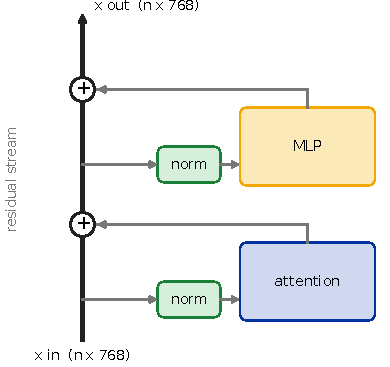
\includegraphics[width=\linewidth]{blk_block.pdf}
    \column{0.56\textwidth}
      \vskip 8pt
      {\small
      \textbf{Attention}: tokens exchange information. The \emph{only} place in the block where
      tokens see each other.
      \vskip 5pt
      \textbf{MLP}: each token alone; two thirds of the weights.
      \vskip 5pt
      \textbf{Norm} before each, and the result \textbf{added back}: LayerNorm from [44], the
      residual connection from [50].}
      \vskip 6pt
      \keybox{Every piece but attention is something you already met. GPT-2's order: norm,
      sublayer, add.}
  \end{columns}
\end{frame}

\begin{frame}{The residual stream is the real object}
  \vskip 6pt
  Read the block as a \textbf{stream} of token vectors running straight through the network, and
  each sublayer \emph{writing an update into it}:
  \vskip 8pt
  \begin{center}
    $\mathbf{x} \leftarrow \mathbf{x} + \text{Attention}\big(\text{LN}(\mathbf{x})\big)$
    \qquad then \qquad
    $\mathbf{x} \leftarrow \mathbf{x} + \text{MLP}\big(\text{LN}(\mathbf{x})\big)$
    \qquad {\small (LN = LayerNorm)}
  \end{center}
  \vskip 6pt
  \takebox{The stream itself is never normalised: each sublayer reads a normalised copy and adds
  a \textbf{correction}. Gradients reach the early layers along the stream - the ResNet argument
  from [50] - and a token's vector gathers meaning layer by layer.}
  \vskip 6pt
  {\scriptsize\color{gray} GPT-2 moved the norm ``to the input of each sub-block'' (Radford et al.,
  2019). The 2017 paper normalised after the add: $\mathbf{x} \leftarrow
  \text{LN}(\mathbf{x} + f(\mathbf{x}))$.}
\end{frame}

\begin{frame}{By hand: LayerNorm on creature}
  \vskip 4pt
  LayerNorm ([44]) rescales one token's vector so its numbers have mean 0 and spread 1. Creature
  after LLM-3, $(0,\ 0.47,\ 0.47,\ 2.13)$:
  \vskip 6pt
  \begin{center}
  \begin{tabular}{ll}
    mean & $(0 + 0.47 + 0.47 + 2.13)/4 = 0.77$ \\[2pt]
    spread & $\sqrt{\tfrac{1}{4}\sum (x_i - 0.77)^2} = 0.81$ \\[2pt]
    normalised & $(x - 0.77)/0.81 = (-0.95,\ -0.37,\ -0.37,\ 1.68)$ \\[2pt]
    then & times a learned scale, plus a learned shift (1 and 0 here) \\
  \end{tabular}
  \end{center}
  \vskip 8pt
  \keybox{Each token is normalised on its own numbers - not across the batch, as BatchNorm does
  ([44]). So it works the same for one sentence or a thousand.}
\end{frame}

\begin{frame}{Masking: a decoder must not read the future}
  \vskip 4pt
  A model trained to predict the next token must not be allowed to look at it. The fix is one
  line: add $-\infty$ above the diagonal \emph{before} the softmax.
  \vskip 6pt
  \begin{center}
    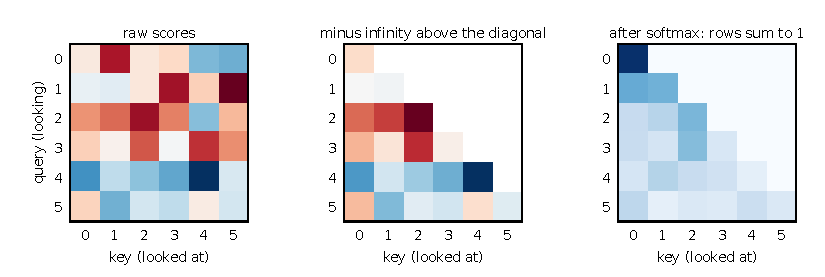
\includegraphics[width=0.92\linewidth]{blk_causal_mask.pdf}
  \end{center}
  \vskip -2pt
  {\small $e^{-\infty} = 0$, so those weights become \textbf{exactly} zero, and each row still sums
  to one.}
\end{frame}

\begin{frame}{By hand: the mask on creature's grid}
  \begin{columns}[T]
    \column{0.46\textwidth}
    \small
    LLM-3's grid (queries read ``noun'', keys read ``adjective''), now with the mask:
    \begin{itemize}
      \item fluffy sees only itself: $(1, 0, 0)$;
      \item blue sees fluffy and itself, scores $0, 0$: $(0.5, 0.5, 0)$;
      \item creature's row does not change: $(0.47, 0.47, 0.06)$.
    \end{itemize}
    \vskip 4pt
    Its adjectives came first, so the mask took nothing from it.
    \column{0.52\textwidth}
    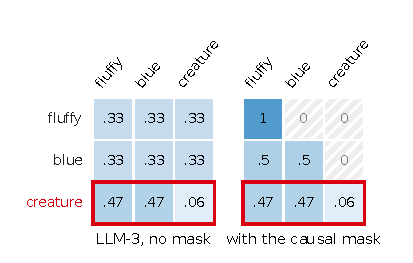
\includegraphics[width=\linewidth]{blk_mask_grid.pdf}
  \end{columns}
  \vskip 6pt
  \takebox{In English adjectives come before their noun, so a left-to-right model can still let
  the noun gather them. What the mask removes is the other direction.}
\end{frame}

\begin{frame}{Why that trick matters more than it looks}
  \vskip 10pt
  Without masking you would train on one prediction at a time: feed the first $t$ tokens,
  predict token $t{+}1$, repeat.
  \vskip 10pt
  With masking, one forward pass over $n$ tokens gives \textbf{$n$ training signals at once}:
  every prefix is predicted at the same time, and none of them can cheat.
  \vskip 12pt
  \keybox{A large part of why pretraining on internet-scale text is affordable at all. The causal
  mask is not a safety measure; it is a \textbf{throughput} decision that happens to enforce
  correctness. (LLM-5 and LLM-7 come back to it.)}
\end{frame}

\begin{frame}{Modern block recipe}
  \vskip 8pt
  The block has been tuned since 2017. Three changes you will meet in current models:
  \vskip 8pt
  \begin{center}
  \footnotesize
  \begin{tabular}{lll}
    \toprule
    \textbf{2017} & \textbf{Now} & \textbf{Why} \\
    \midrule
    norm after the add & norm first (GPT-2 already) & trains more stably; can even skip warm-up \\
    LayerNorm & \textbf{RMSNorm} & cheaper: no mean, only the spread \\
    ReLU in the MLP & \textbf{SwiGLU} & a gated MLP; better quality in Shazeer's tests \\
    \bottomrule
  \end{tabular}
  \end{center}
  \vskip 6pt
  {\scriptsize\color{gray} Xiong et al., ICML 2020 (norm first); Zhang \& Sennrich, NeurIPS 2019
  (RMSNorm); Shazeer, 2020 (GLU variants).}
  \vskip 8pt
  \watchbox{None of these changes the story: attention, an MLP, norms and the residual stream.
  LLM-14 opens a 2026 model card and finds the same block.}
\end{frame}

\begin{frame}{Now stack it}
  \begin{columns}[T]
    \column{0.5\textwidth}
      \vskip -4pt
      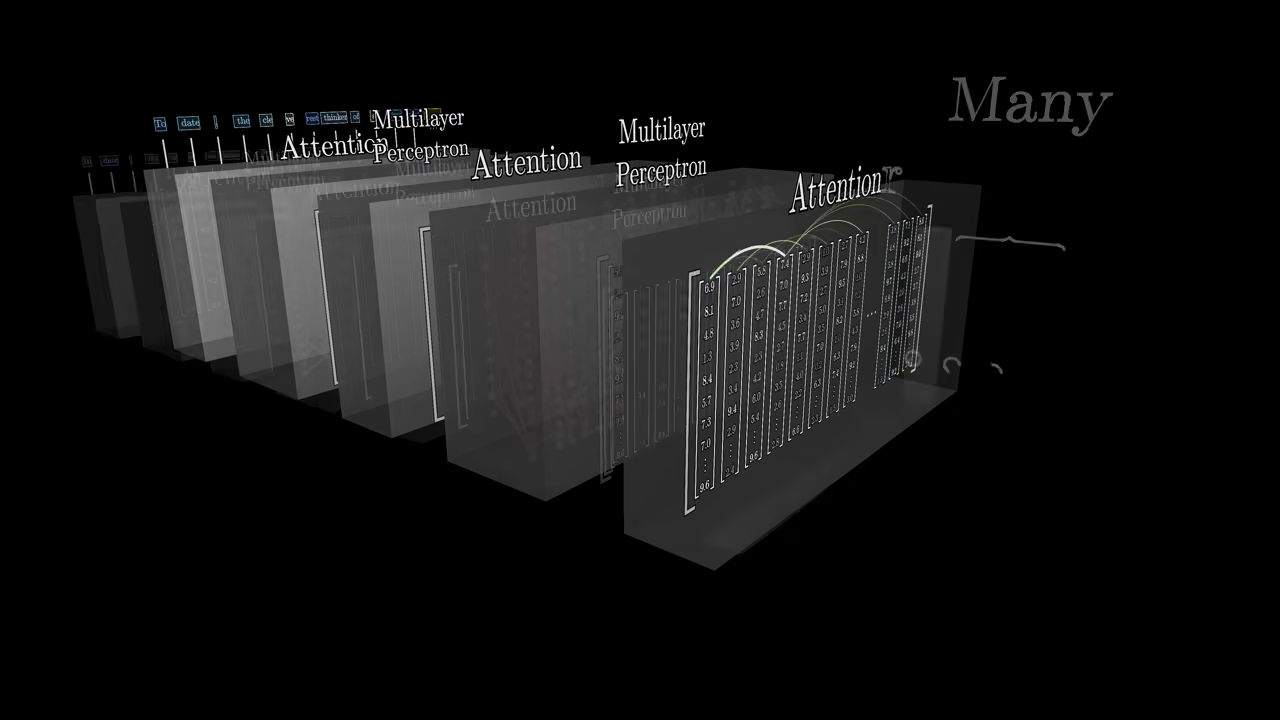
\includegraphics[width=\linewidth]{deep_stack.png}\\ \bbb
    \column{0.47\textwidth}
      \vskip 8pt
      {\small A block takes $n \times 768$ numbers in and gives $n \times 768$ out - the same
      shape, which is why blocks can be stacked. GPT-2 small stacks \textbf{12}.
      \vskip 8pt
      Each block alternates \textbf{tokens talking} (attention) with \textbf{each token thinking
      alone} (the MLP).
      \vskip 8pt
      A token's vector starts as ``the word \emph{creature}'' and, layer by layer, gathers what
      the context implies: fluffy, blue, cute, and whatever comes next.}
  \end{columns}
  \vskip 4pt
  \takebox{Same block, 12 times. That is the whole architecture.}
\end{frame}

\begin{frame}{Where GPT-2's 124M live}
  \begin{center}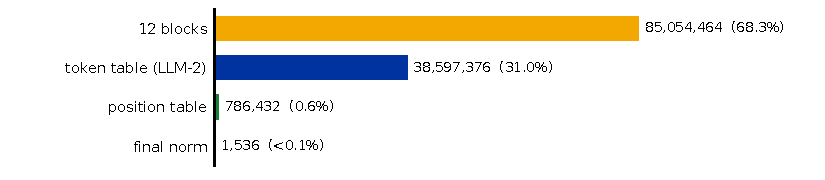
\includegraphics[width=0.94\linewidth]{blk_params_124m.pdf}\end{center}
  \vskip -2pt
  {\small $12 \times 7{,}087{,}872 = 85{,}054{,}464$ in the blocks; the token table (LLM-2's 31\%);
  1{,}024 learned positions; one final norm. Total \textbf{124{,}439{,}808}, read from the weight
  file.}
  \vskip 6pt
  \keybox{Two thirds of every block is MLP, and the blocks are two thirds of the model. Attention,
  the star of LLM-3, is under a quarter of GPT-2 (22.8\%).}
\end{frame}

% ============================================================ RECAP
\begin{frame}{Recap}
  \vskip 4pt
  \small
  \begin{itemize}
    \item \textbf{Many heads}: $h$ questions at once, each in a smaller space (GPT-2: $12 \times
      64 = 768$), mixed by $W_O$. Real heads: one looks one token back, one sends creature to
      fluffy, many park on the first token.
    \item \textbf{Still blind to order}: one head or twelve, so positions come in before the first
      layer (LLM-2).
    \item \textbf{The MLP}: rows ask, ReLU gates, columns add. A neuron can fire on ``fluffy AND
      creature'', and facts like Messi's sport seem to live here. Two thirds of every block.
    \item \textbf{The block}: norm, attention, add; norm, MLP, add. The stream is never
      normalised; every sublayer writes a correction.
    \item \textbf{The mask}: no reading the future, and $n$ training signals per pass.
  \end{itemize}
\end{frame}

\begin{frame}{Next on the map}
  \begin{center}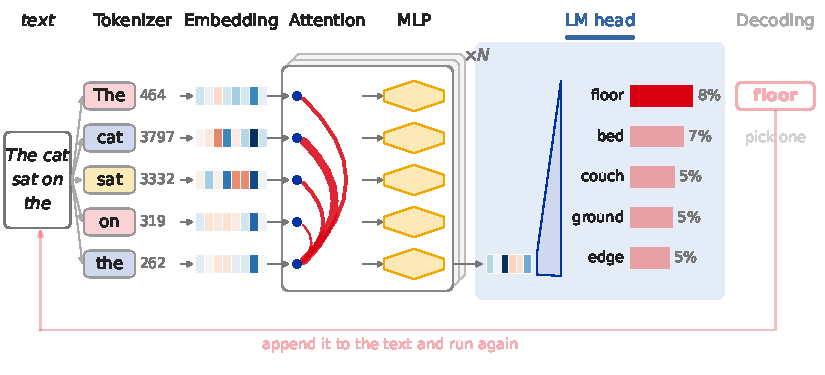
\includegraphics[width=\linewidth]{roadmap_transformers_pass.pdf}\end{center}
  \vskip -2pt
  {\small Next (LLM-5): what comes out at the far end, and three ways to wire the same block.}
\end{frame}

\end{document}

% ============================================================================
% Provenance
%
% PLAN: ml/14_llms/ATTENTION_CHAPTER_PLAN.md, section "L25", approved by the instructor
% 2026-07-19. Frame order follows that outline; the optional "modern block recipe" frame was
% kept rather than cut.
%
% SOURCES:
%   - misc/dl4nlp/02_transformers.tex - multi-head, positional encoding, the block, and the
%     modern-variant table were adapted from it (already in the house palette).
%   - 3Blue1Brown Ch5/Ch6, transcripts in research/, frames in fig/borrowed/3b1b/ with a
%     manifest. Used: multihead.png, attn_mlp_flow.png, deep_stack.png, single_head_full.png.
%     Credit line only, per the instructor's 2026-07-21 decision (no licence tag).
%   - Vaswani et al. (2017) for the PE formula; the architecture figure itself is used in L26.
%
% FIGURES - py_src/l25_l26_figs.py and py_src/l25_real_attention.py:
%   REAL (every number quoted on a slide comes from these scripts' logs):
%     l25_permutation    - the same three tokens in two orders give per-token outputs differing
%                          by 1.1e-16 without positional encoding, and 1.797 with it. The script
%                          RAISES if the no-PE gap exceeds 1e-9, so the deck's central claim in
%                          section 2 cannot silently become false.
%     l25_pe_heatmap     - the sinusoidal matrix, computed from the formula on the slide.
%     l25_pe_dotprod     - PE similarity depends on offset not absolute position; the curves for
%                          positions 10/25/40 agree to within 0.0000.
%     l25_causal_mask    - masked attention pays exactly 0.000 to future tokens; script asserts it.
%     l25_real_heads     - REAL attention weights pulled from intfloat/multilingual-e5-small
%     l25_head_entropy     (12 layers x 12 heads) on the 3b1b running sentence, so the chapter
%                          keeps one example from L24's single head through to multi-head.
%                          Layer 6: sharpest head 1 (entropy 0.92), most diffuse head 0 (1.85).
%   ILLUSTRATIVE (labelled "schematic" on the figure itself):
%     l25_block          - the block as a data-flow diagram.
%
% DELIBERATE CHOICES:
%   - The permutation result is the section-2 predict-first payoff. It is stated as a proof
%     ("not slightly different - identical") because it is one: the mechanism has no term in i
%     or j, which the following frame spells out.
%   - The "what heads learn" frame carries an explicit warning that the labels are our
%     interpretation, not measured. The measured claim is the entropy spread on the frame before.
%   - RoPE and ALiBi are named in one line and not derived, per the plan.
%
% NOT DONE:
%   - No homework frame (house rule: homework lives on the chapter .qmd).
%   - Cross-attention is deferred to L26, where it belongs with the encoder-decoder family.
%   REVISION 2026-10-04: two "Where we are" frames after the title (one forward pass; the life
%   of a model) and "Next on the map" before the closing frame (fig/roadmap_block_pass/_life.pdf,
%   roadmap_transformers_pass.pdf from py_src/llm_roadmap.py; DECISIONS #67).
%   RENAMED 2026-10-05 (DECISIONS #71, the chapter renumbered in teaching order): L25_transformer_block.tex -> LLM4_transformer_block.tex.
%   Labels in the body were renumbered by script; this provenance block keeps the old names.
%   RESTRUCTURED 2026-10-05 (critique, two interview rounds and follow-ups, and the outline in
%     LLM4_transformer_block_OUTLINE.md and LLM_CHAPTER_PLAN.md). Cold open on GPT-2's real fact
%     completions (Messi stored; Mkhitaryan missing; Ella Fitzgerald and Elliott Smith missed to
%     different degrees - people picked by the instructor after three probe runs). Sections: Many
%     heads; The MLP: where facts live (the 3b1b chapter-7 stills extracted in July for this, now
%     used); The block (GPT-2's norm-first order). Cut: the Position section except one proof frame
%     (LLM-2 owns position, #68; the sinusoid frames carried wrong extrapolation claims), the
%     "Where we got to" recap, attn_mlp_flow, the "You can now build one" ending; the e5 real heads.
%     New, from py_src/block_figs.py (toy numbers asserted; --gpt2 = one run of the cached GPT-2:
%     probes, name tokens, attention of every head on the creature sentence, parameter counts from
%     the safetensors header): blk_fact_probes, blk_two_heads (one number per head), blk_gpt2_entropy
%     and blk_gpt2_heads (layer 5 head 11 = previous token, weight 1.00; layer 6 head 2 = creature
%     -> fluffy .62; an attention-sink head; 39 of 144 heads > 90% on the first token),
%     blk_neuron (fluffy AND creature -> the new "cute" slot), blk_params_block (MLP 66.6%),
%     blk_params_124m, blk_block (norm first), blk_mask_grid. Callbacks re-pointed to the current
%     decks: LayerNorm and BatchNorm [44], residual [50], the MLP [41] (July said L14/L15/L17).
%     Notation W_Q, W_K, W_V, W_O (subscripts, as LLM-3). Sources checked: GPT-2 paper ("moved to the
%     input of each sub-block"); Xiao et al. (attention sinks), Geva et al. 2021, Meng et al. 2022,
%     Kandpal et al. 2023, Xiong et al. 2020, Zhang & Sennrich 2019, Shazeer 2020 cited from memory
%     of the papers - recheck venues before delivery.
%     Build fixes: "Stored, half-stored, missing" and "Three real heads" each split in two ("So where
%     does a fact live?", "Attention sinks" with blk_gpt2_sink, the first-token share per layer);
%     l25_permutation and l25_causal_mask (drawn 9+ in wide, text 3.6-4.7 pt on the slide) ported
%     into block_figs.py at slot size as blk_permutation (1.1e-16 reproduced, asserted) and
%     blk_causal_mask. 41 pages; 0 errors, 0 overflow, 0 footer collisions, 0 small text, 0 clipping
%     flags. No student review yet (needs the instructor's OK).
%     Self-review round (2026-10-05, instructor back): GPT-2's MLP uses GELU, not ReLU (config
%     "gelu_new") - one line on the ReLU frame; Meng et al. edited GPT-2 XL; "the first token,
%     whatever it is" narrowed to this sentence's "a"; the attention-sink reason marked as the usual
%     explanation; "attention is about a fifth of GPT-2" -> "under a quarter (22.8%)", asserted in
%     block_figs.py; "today's answer" hedged like the evidence frame; LN spelled out; the three
%     real-head titles split over two lines (they ran into each other).
% ============================================================================
